\chapter{目标物体位姿数据库生成研究}
\label{cha:dataset}
\section{引言}
\label{sec:chap03:intro}
现有的目标物体位姿数据库多为研究人员公开的数据集,这类数据集按照生成方式可分为两种:一种是通过人工测量的方法得到真实场景图片中的物体位姿,另一种是使用计算机渲染的方法将物体叠加在真实场景图片中,通过提前设定
虚拟物体的运动轨迹,以得到每一帧图片中物体相对于相机的位姿。第一种方式的数据量较大,包含多种环境及光照下的图片,并利用人工对齐或者陀螺仪测量的方法得到物体相对于相机的位姿,比如~ObjectNet 3D\cite{XiangObjectnet3dLargeScale2016}~数据库、~ACCV~数据库\cite{HinterstoisserGradientResponseMaps2012}、~ICVL~数据库\cite{DoumanoglouRecovering6DObject2015}等。
但这类方法无法保证数据库真值的可靠性,其位姿获取方法是通过将物体的轮廓模型与图像进行人为对齐,以得到物体的位姿,该方法使用的对齐模型与实际物体存在一定差异,仅匹配物体的轮廓信息而忽略细节差异,
因此并不适用于本文所提出的目标物体模型与场景边缘图像的精确匹配算法,无法用于精度测试以及算法的训练。第二种方法通过计算机渲染将目标物体的虚拟图像叠加于真实图片中,该方法能够预先设定目标物体运动的轨迹以及姿态得到
位姿真值,或通过渲染引擎以计算目标物体的精确位姿,比如~ISY~数据库\cite{VikstenComparisonLocalImage2009}、~Rigid Pose~数据库\cite{PauwelsRealTimeModelBasedRigid2013}等,但现有数据库较多是针对普通物体,对于贫纹理物体的相关数据库非常稀少,数据量无法达到要求,且虚拟物体与真实场景图像间的过度存在较大失真,
边缘提取算法可能将过度处的锯齿识别为场景边缘,导致系统误差,因此也并不适用于本文的算法。由于物体相对于相机坐标系的位姿难以精确测量,真实场景的位姿数据库构建十分困难,需要耗费大量资源。目标追踪领域已有大量的研究以及文章,然而绝大多数文章注重于描述算法,对其使用的
数据并不公开或者只提供部分样本数据,达不到用以训练模型或者复现文中算法的效果,这在一定程度上阻碍了研究的发展。

本文将利用机器学习的方法实现目标物体的检测以及姿态回归,完成追踪算法的自动初始化。因此需要构建目标物体检测以及回归数据库,用以作为训练样本提供给相关算法,针对这一问题,本文将使用第~\ref{cha:model_based_tracking}~章中提出的算法对
贫纹理目标物体实现位姿追踪,并对结果进行判定。使用追踪成功的视频生成样本数据,该数据库将被用于训练物体的检测以及姿态回归模型,由于该数据库是由真实场景采集的图像生成,因此相比于虚拟渲染的视频数据更具有真实性,能够使得后续模型对真实环境的适应性更强,提高系统对真实场景中存在的干扰及噪音的鲁棒性。
其次,由于真实场景的目标物体位姿难以测量,因此为实现本文目标物体位姿追踪算法的精度测试,本章还将研究利用计算机渲染技术生成虚拟视频的方法,通过渲染引擎获得图片中目标物体相对于相机的精确位姿关系,构成精度测试数据库,利用该数据库对算法的精度进行定量测试。

\section{训练数据库生成}
\label{sec:train_dataset}
第~\ref{cha:model_based_tracking}~章中提出的追踪算法需要给定首帧图像中,物体的初始化位姿。本文在研究追踪算法时,通过手动配准的方式得到该位姿,使得算法不能自行启动并运行。
本文在后续章节拟使用机器学习的方法实现目标的检测以及姿态回归,实现目标物体在首帧图像中的自动检出以及姿态估计,为追踪算法提供初始化位姿。
本节将研究构建目标物体的图像以及位姿数据库,以备初始化系统的模型训练,以完成目标检测以及姿态回归算法。本文将使用前述追踪系统对真实场景的图像进行追踪,使用光栅点权值构造追踪效果的评价函数,
保存追踪效果良好的图像,并记录相关帧图像中目标物体相对于相机坐标系的位姿真值,以备后续使用。由于目标检测与姿态回归为两个单独的模型,因此需要建立的数据库有两个,分别对应目标物体的图像位置检测以及位姿的回归。
\subsection{目标物体及采集设备选择}
\label{sec:dataset_model}
本文的研究目标是贫纹理物体,通过寻找三维模型与场景图像的最优匹配,以解算位姿。针对研究背景,本文需要寻找工业现场较为常见的一些目标物体作为实验对象,由于模型的复杂度将影响系统的精度以及抗干扰力,为测试算法对不同模型的检测以及追踪的鲁棒性,
本文选择模型的复杂度、光泽和大小都不同的贫纹理物体作为实验对象,构造数据库。对于简单的模型,
其图像边缘较为明显,对于背景的小幅干扰以及图像噪音鲁棒性较高,但当场景中出现与模型边缘平行的背景边缘时,算法将容易出现误匹配,因此需要选择一定数量的简单模型,以测试追踪算法对该类问题的抗干扰能力;对于复杂的模型,其边缘往往由较短的线段构成,且边缘线段的数量较多,
这将对边缘提取的精度提出挑战,能够正确有效地提取到所有可视范围内的物体边缘,成为算法的主要难点,但复杂物体由于边缘信息丰富,对于模型匹配的方法,其成功率将有所提高。类比于特征点匹配方法,当特征点丰富时,匹配的精度以及成功率也会有所提升,对于本文所提算法,物体的边缘即相当于特征点,因此
模型边缘较多时,能够提高追踪算法的成功率。

模型的多样性以及复杂度同样影响检测算法的效果。首先由于检测算法将使用机器学习对图像进行分类,因此模型的差异性需要较为明显,否则图像特征过于相似将导致分类的误判率较高。
其次,为降低检测算法的误判率,需要利用较为简单的物体加入训练,因为容易出现与简单模型的图像信息相似的背景信息,若算法能够正确检测到该类物体,且背景误判率较低,则说明检测算法以及提取到的图像特征
能够很好地区分目标物体与背景边缘。模型的对称性会对姿态的回归造成影响,因为对称的模型会使得物体旋转一定角度后的图像特征与旋转前相同,导致其位姿真值变化后,图像特征不变,这将引起回归算法的误差,后续将针对该问题进行详细研究。

基于以上考虑,本文选定如图~\ref{fig:chap03:object_model}~所示的~4~种目标物体,其中包含圆盘固定件、飞机模型、螺母以及五边形球体。其中圆盘固定件、螺母属于较为简单的模型,其边缘数量少,含有长度较长的模型边缘,在
边缘提取时比较明显,但也由于边缘特征较为简单,更易于出现与该类物体类似的背景边缘,在使用机器学习算法进行检测时易发生误检;而飞机模型以及五边形球体属于复杂模型,边缘数量较多,特别是飞机模型,其上含有大量细节信息,机身中部含有较多长度较短的模型边缘,对边缘提取以及匹配算法提出挑战。
使用复杂度不同的目标物体作为研究对象,构建数据库,能够有效提高算法的适用性,以证明算法在多种场景以及目标物体上都能完成检测以及位姿追踪。
\begin{figure}[t] %[h]
  \centering%
  \subcaptionbox{圆盘固定件\label{fig:chap03:san_model}}{%    
    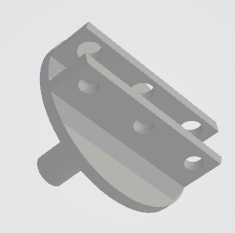
\includegraphics[height=3.5cm]{san_model}\hspace{0.2em}}
  \subcaptionbox{飞机模型\label{fig:chap03:jet_model}}{%    
    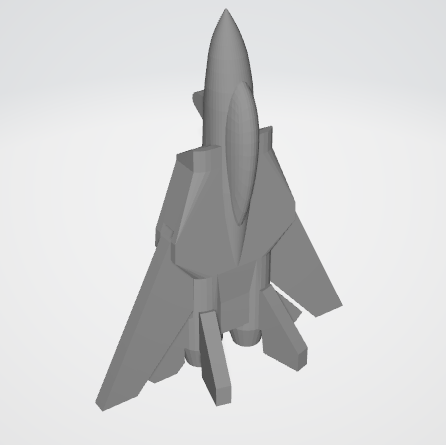
\includegraphics[height=3.5cm]{jet_model}\hspace{0.2em}}
  \subcaptionbox{螺母\label{fig:chap03:nut_model}}{%    
    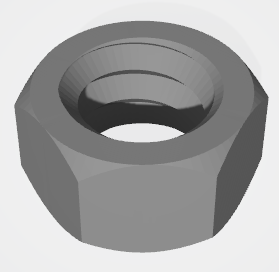
\includegraphics[height=3.5cm]{nut_model}\hspace{0.2em}}
  \subcaptionbox{五边形球体\label{fig:chap03:ball_model}}{%    
    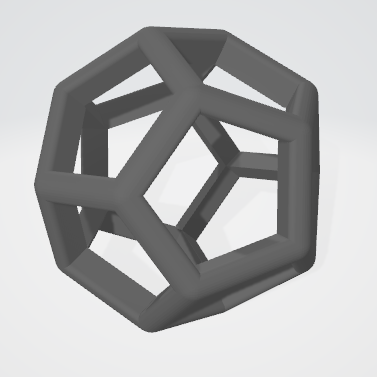
\includegraphics[height=3.5cm]{ball_model}}
  \caption{目标物体模型}
  \label{fig:chap03:object_model}
\end{figure}

\begin{figure}[t] %[h]
\centering%
\subcaptionbox{Basler~工业相机\label{fig:chap03:basler_camera}}{%    
  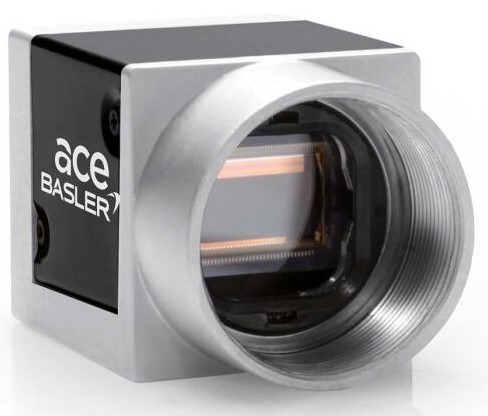
\includegraphics[height=4.5cm]{basler_camera}\hspace{2em}}
\subcaptionbox{工业相机镜头\label{fig:chap03:camera_len}}{%    
  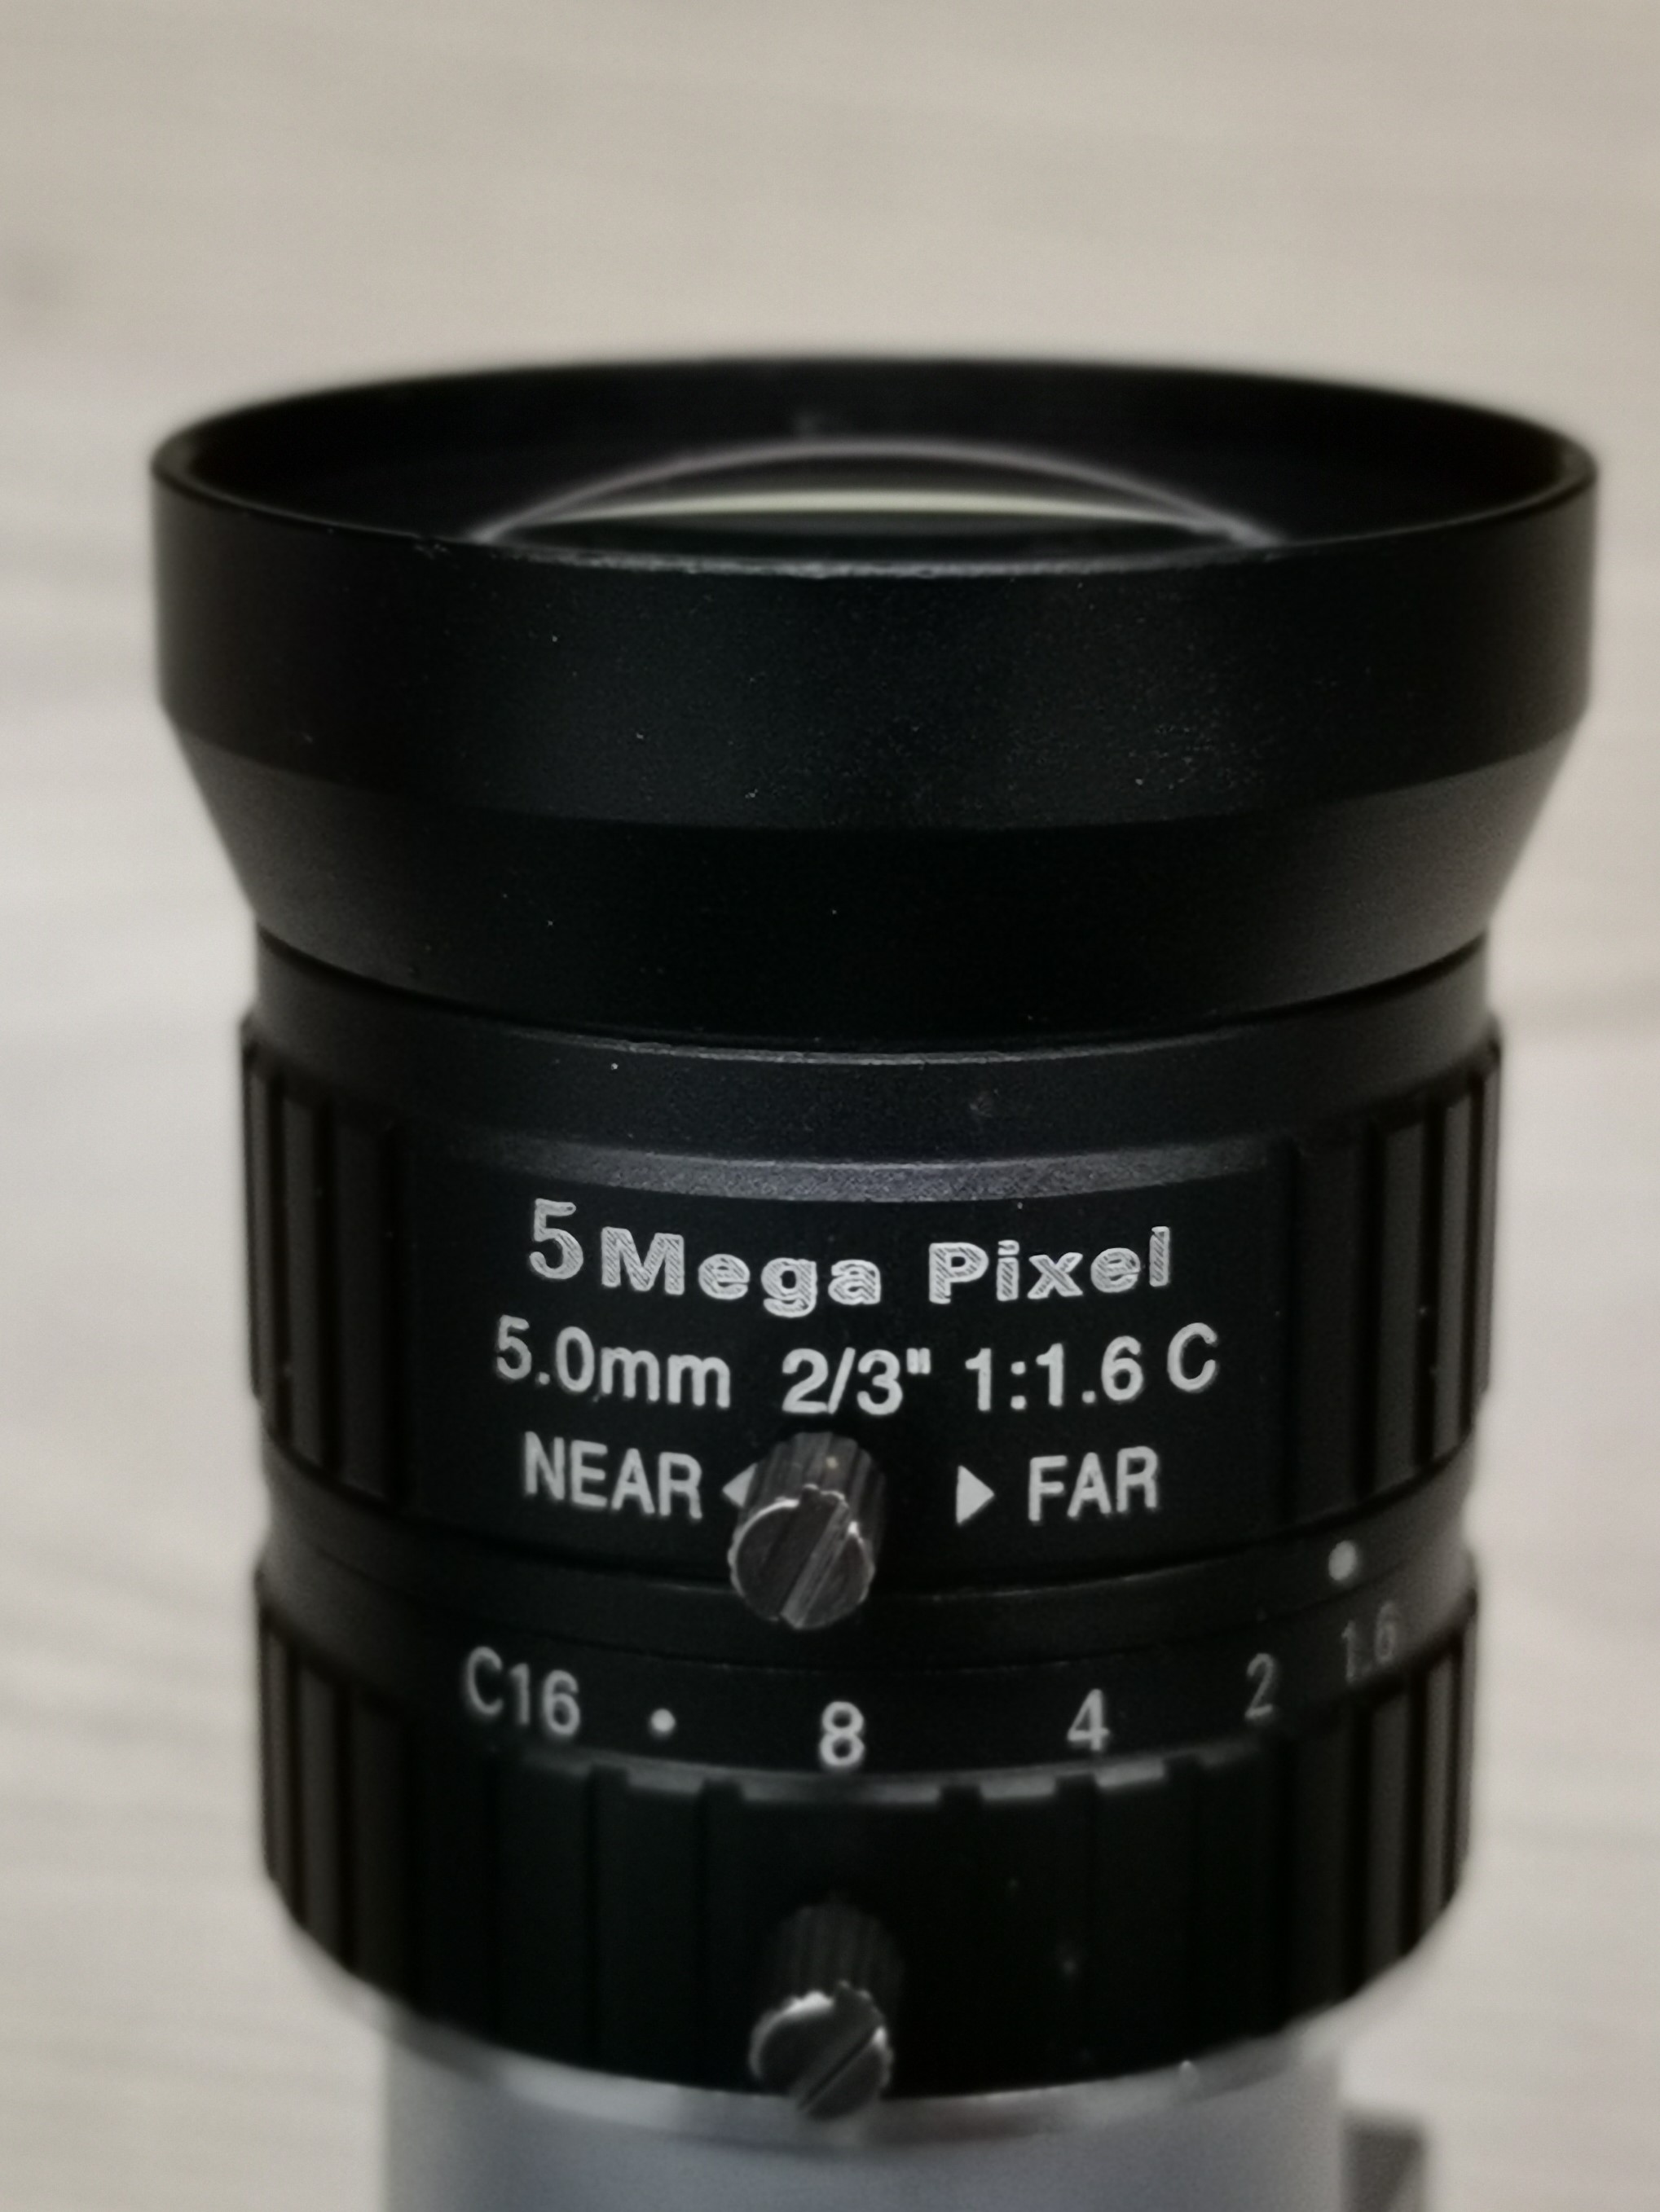
\includegraphics[height=4.5cm]{5mm_len}}
\caption{图像采集传感器}
\label{fig:chap03:camera_len_device}
\end{figure}

本研究使用~Basler(R) acA1300-60gm~相机采集图像,如图~\ref{fig:chap03:basler_camera},该相机最高帧率~60fps,分辨率为~1280*1024,使用~GigE~接口连接上位机,是一款常用于半导体及零部件检测领域的灰度工业相机。该款相机软件驱动完善,能够使用
现有人机交互软件进行参数调整以及视频录制,且完成驱动程序安装后,能够使用代码对其进行设置以及调用。配合使用~5mm~工业定焦镜头,如图~\ref{fig:chap03:camera_len},该镜头进光量能够手动调节,方便对不同光照强度的环境进行模拟。
所用目标物体由高精度~3D~打印技术获得,保证实物与三维模型完全匹配,并且为了模拟工业金属工件的表面光泽,对螺母工件表面进行了喷锡处理。
\subsection{检测数据库}
\label{sec:detect_dataset}
本文将利用图像特征识别与分类的方法对目标物体实现检测,该类方法通过提取图像中的特征以训练模型,使得模型能够正确地区分不同类别的特征输入。由于本文研究目标为贫纹理物体,使得传统特征点的提取方法不再适用,
结合本文提出的基于边缘图像的追踪方法,本文拟使用目标物体的边缘图像特征对模型进行训练,因此使用图像的边缘信息构建检测数据库。

首先通过图像传感器采集大量包含目标物体的灰度视频,在视频中应尽量多的出现目标物体的各种位姿,如图~\ref{fig:chap03:raw_gray_imgs}~所示。为提高算法的鲁棒性,本文使用含有较多边缘信息的背景图片,以模拟复杂环境对系统的影响。
之后对采集到的视频,使用追踪算法以获取每一帧图像中目标物体的位姿,通过该位姿信息以及物体模型,能够将模型光栅点映射于图像平面。之后遍历所有光栅点的图像坐标~$(x_i,y_i)$,寻找模型光栅点中的坐标极值点,即
所有点坐标中的~$min\_x,~max\_x,~min\_y,~max\_y$,由此能够确定一个图像矩形范围,该范围的左顶点为~$P(min\_x,~min\_y)$,长宽为~$(leng\_x,~leng\_y)$,其中~$leng\_x=max\_x-min\_x,~leng\_y=max\_y-min\_y$。
通过该坐标范围确定目标物体在图像中的位置,该区域内的图像特征即为目标物体的图像特征,如图~\ref{fig:chap03:area_interesting}~所示。

\begin{figure}[b] %[h]
  \centering%
  %%\subcaptionbox{目标物体图像区域\label{fig:chap03:area_interesting}}[\linewidth]{%    
    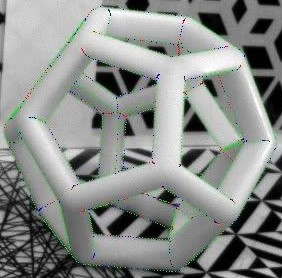
\includegraphics[height=2cm]{ball_jiequ_1}\hspace{0.5em}
    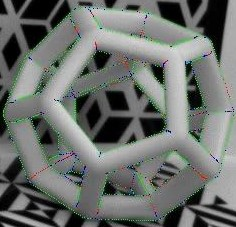
\includegraphics[height=2cm]{ball_jiequ_2}\hspace{0.5em}
    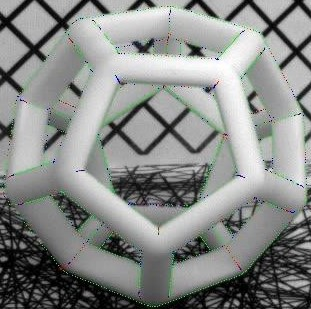
\includegraphics[height=2cm]{ball_jiequ_3}\hspace{0.5em}
    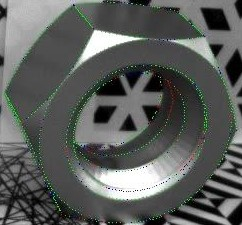
\includegraphics[height=2cm]{nut_jiequ_1}\hspace{0.5em}
    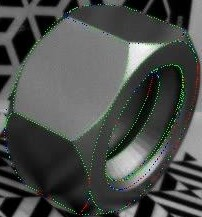
\includegraphics[height=2cm]{nut_jiequ_2}\hspace{0.5em}
    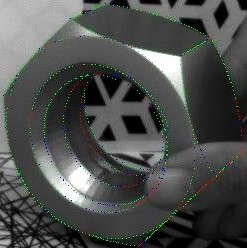
\includegraphics[height=2cm]{nut_jiequ_3}
    \vskip 1pt
    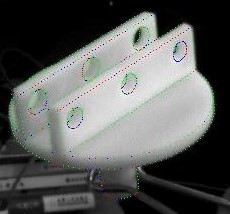
\includegraphics[height=1.8cm]{san_jiequ_1}\hspace{1em}
    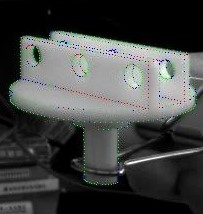
\includegraphics[height=1.8cm]{san_jiequ_2}\hspace{1em}
    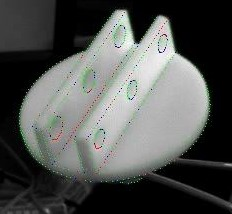
\includegraphics[height=1.8cm]{san_jiequ_3}\hspace{1em}
    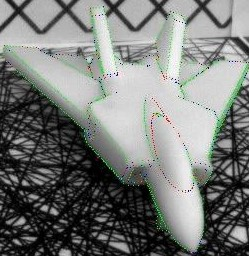
\includegraphics[height=1.8cm]{jet_jiequ_3}\hspace{1em}
    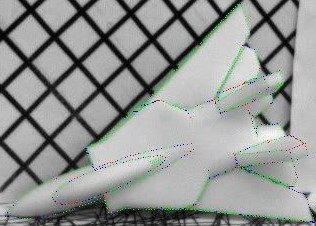
\includegraphics[height=1.8cm]{jet_jiequ_2}\hspace{1em}
    \vskip 1pt
    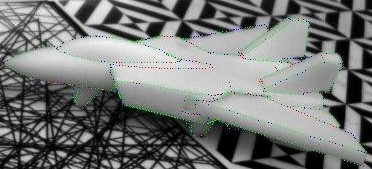
\includegraphics[height=1.8cm]{jet_jiequ_1}
  \caption{分割后的目标物体图像区域}
  \label{fig:chap03:area_interesting}
  \end{figure}

\begin{figure}[t] %[h]
  \centering%
  %\subcaptionbox{原始图像\label{fig:chap03:raw_gray_imgs}}[\linewidth]{%    
    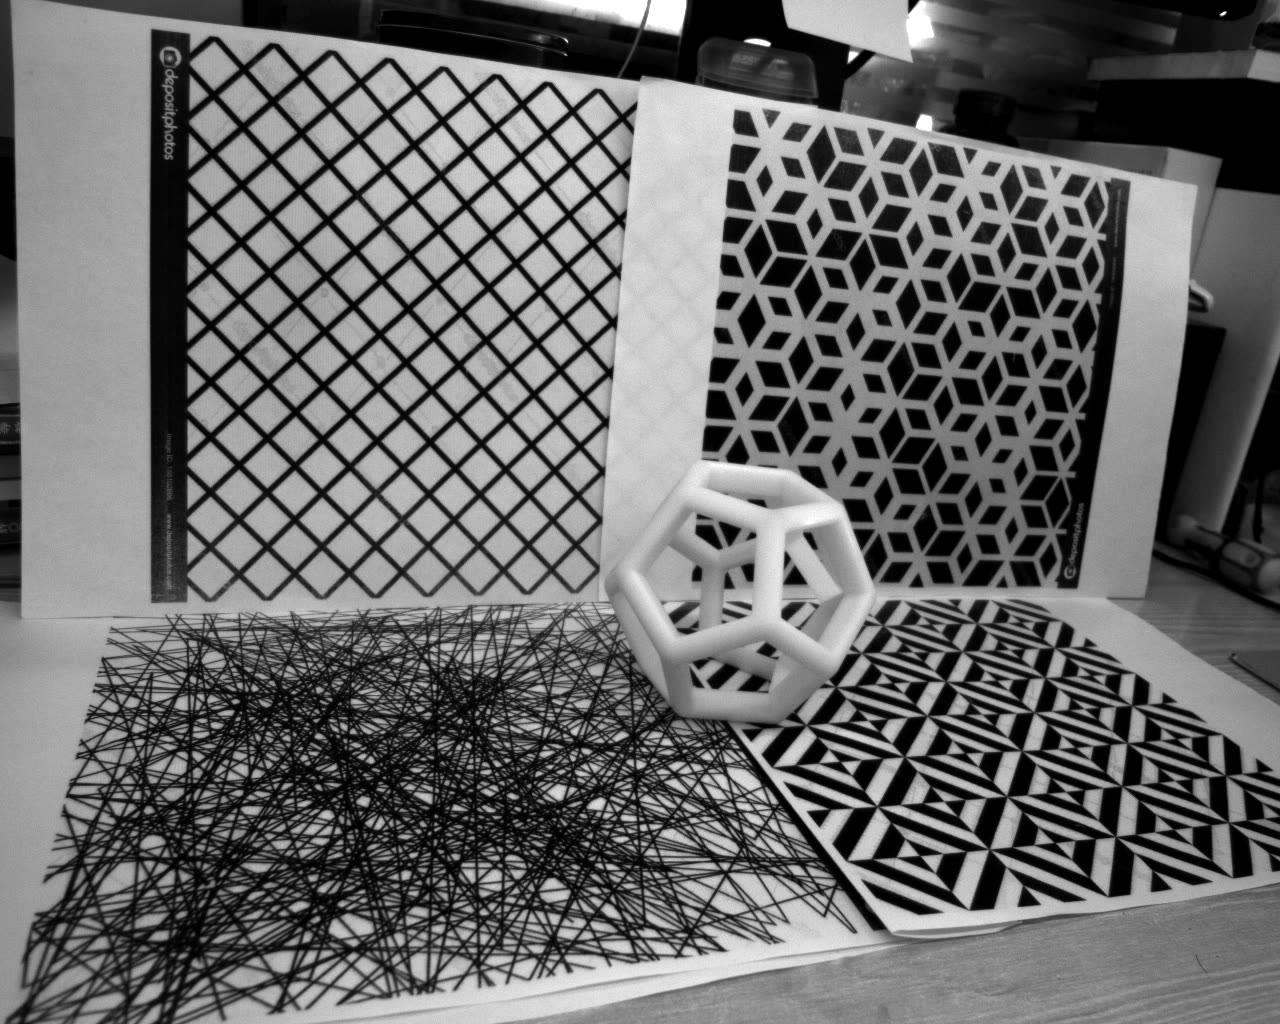
\includegraphics[height=3.8cm]{ball_yuan_1}
    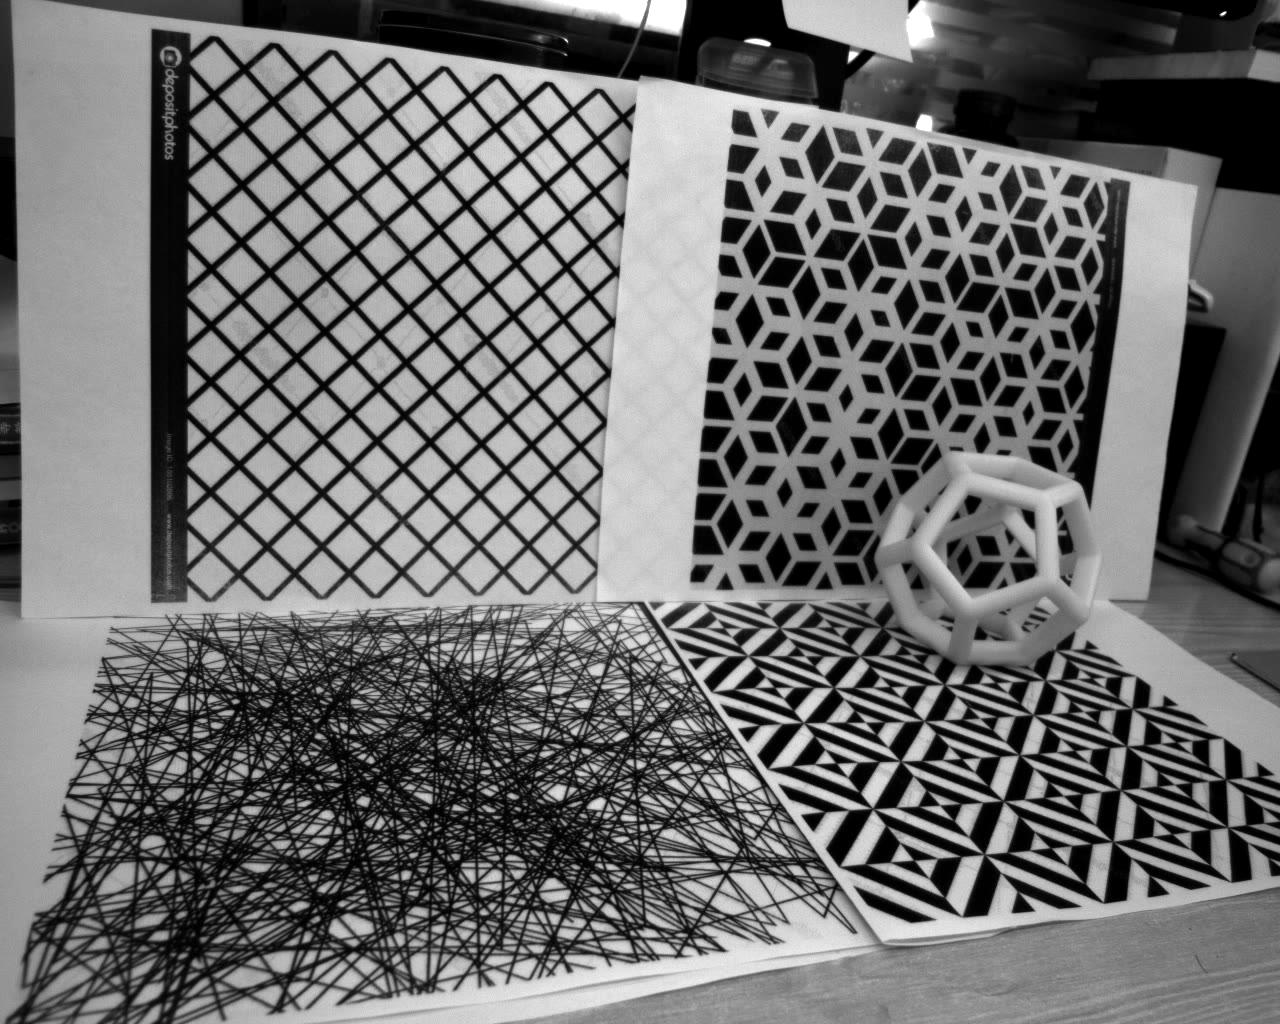
\includegraphics[height=3.8cm]{ball_yuan_2}
    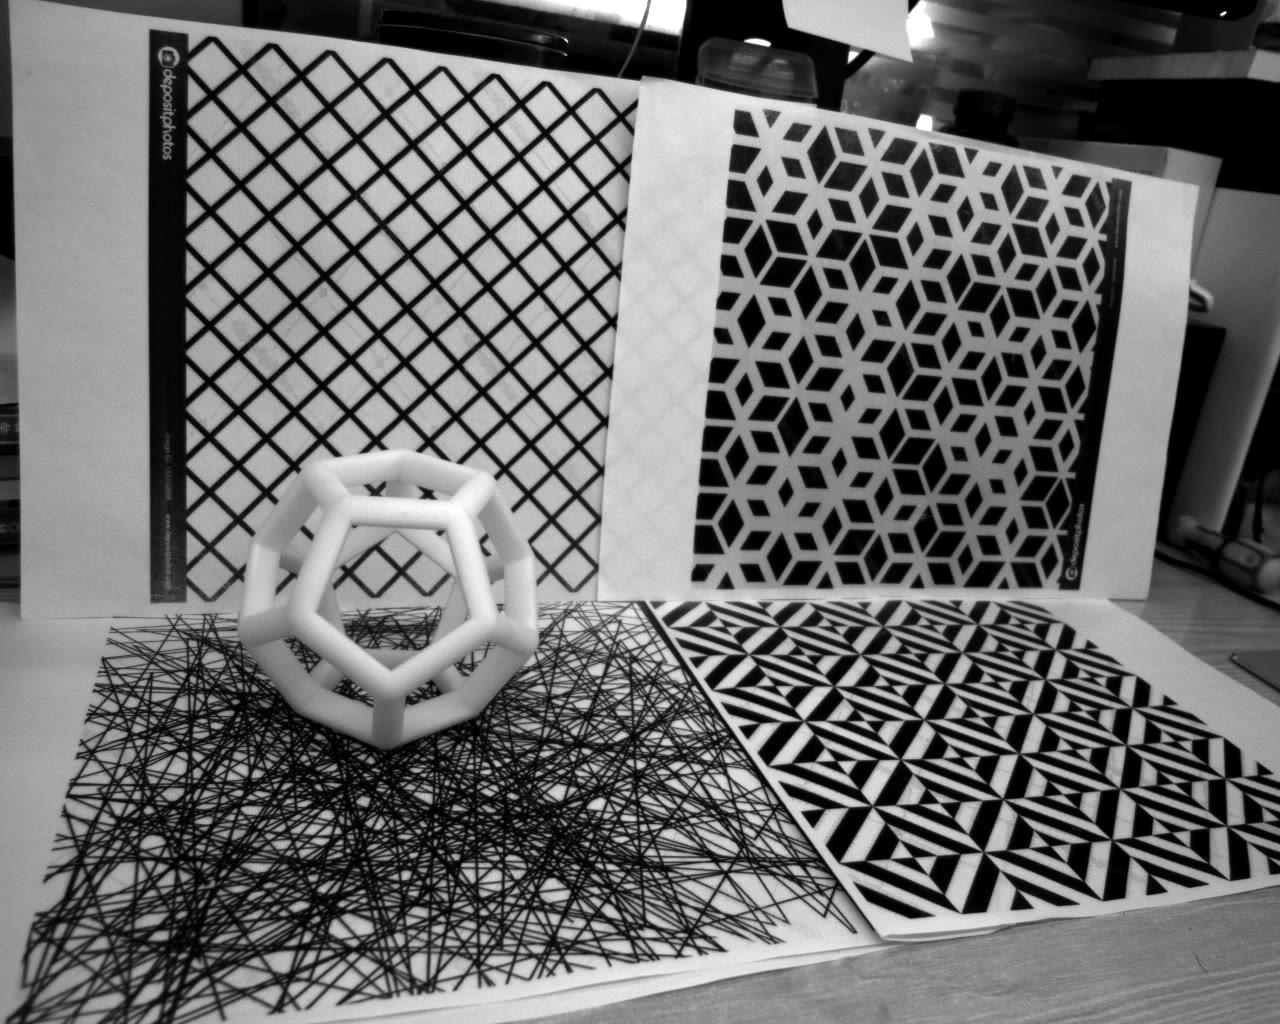
\includegraphics[height=3.8cm]{ball_yuan_3}
    \vskip 1pt
    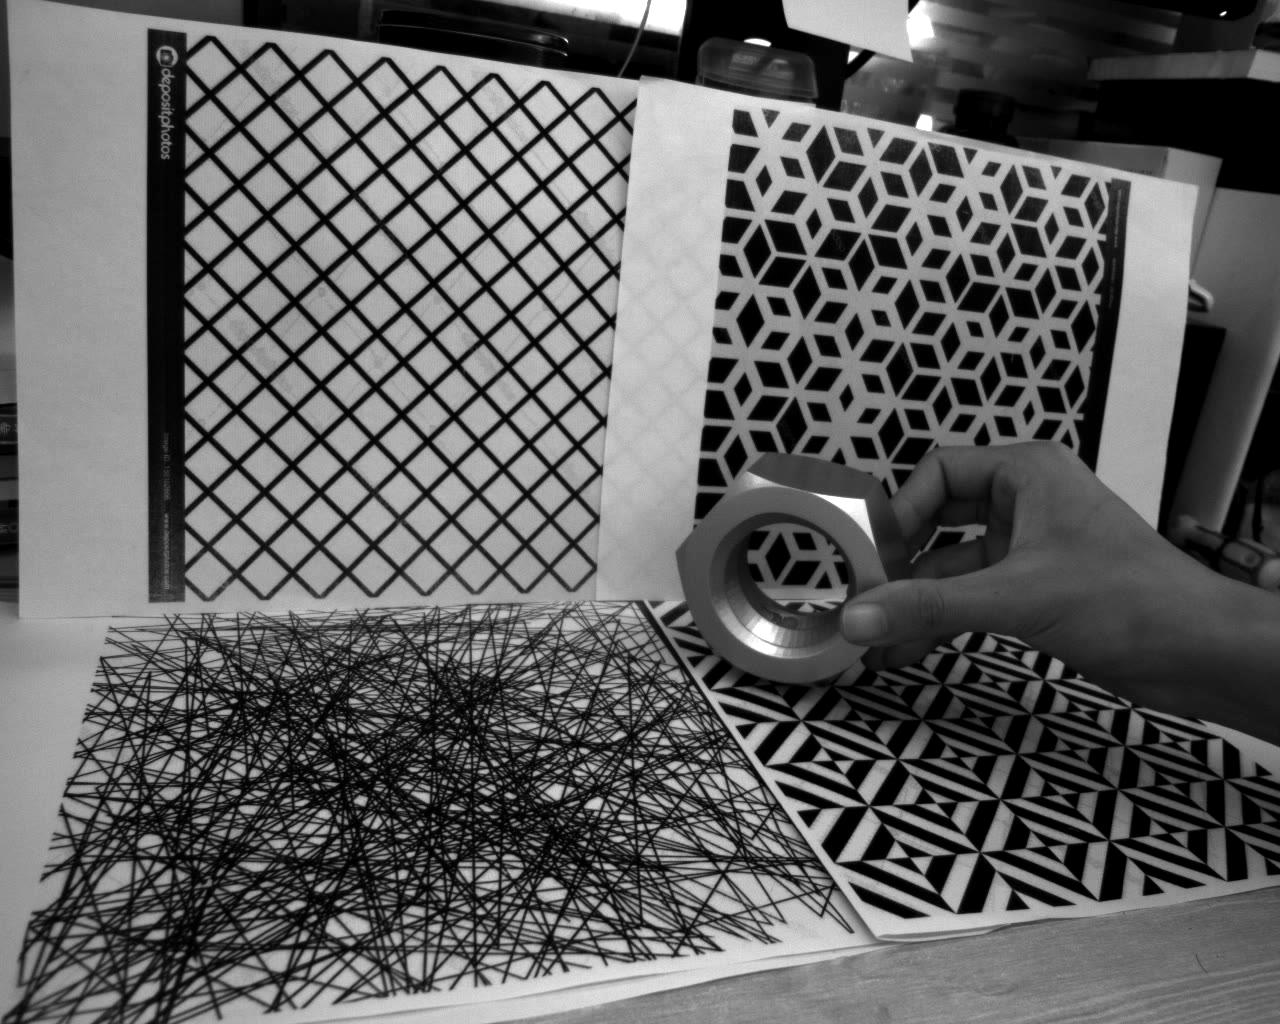
\includegraphics[height=3.8cm]{nut_yuan_1}
    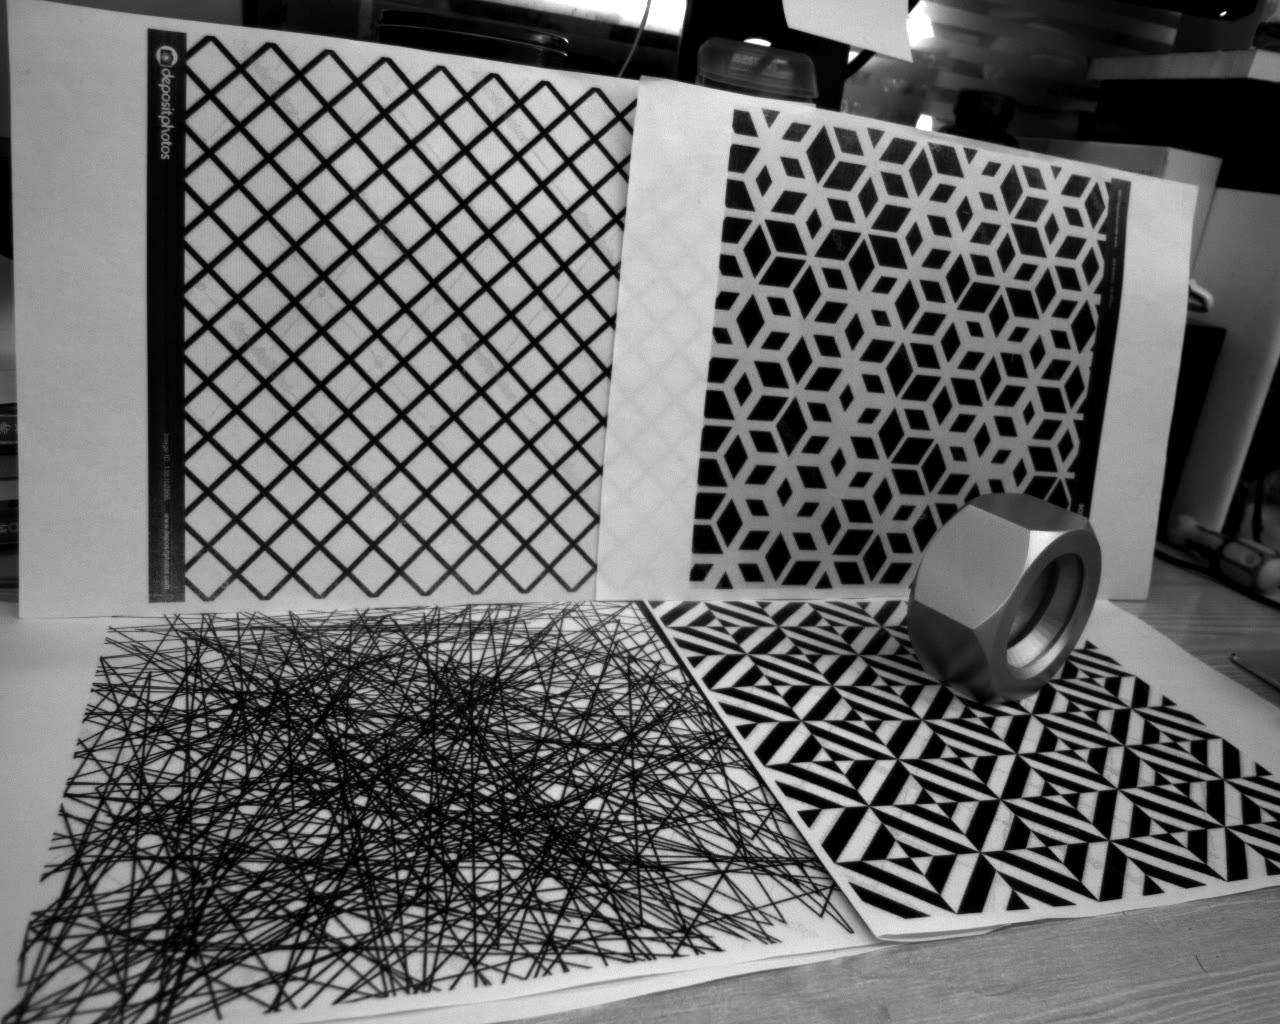
\includegraphics[height=3.8cm]{nut_yuan_2}
    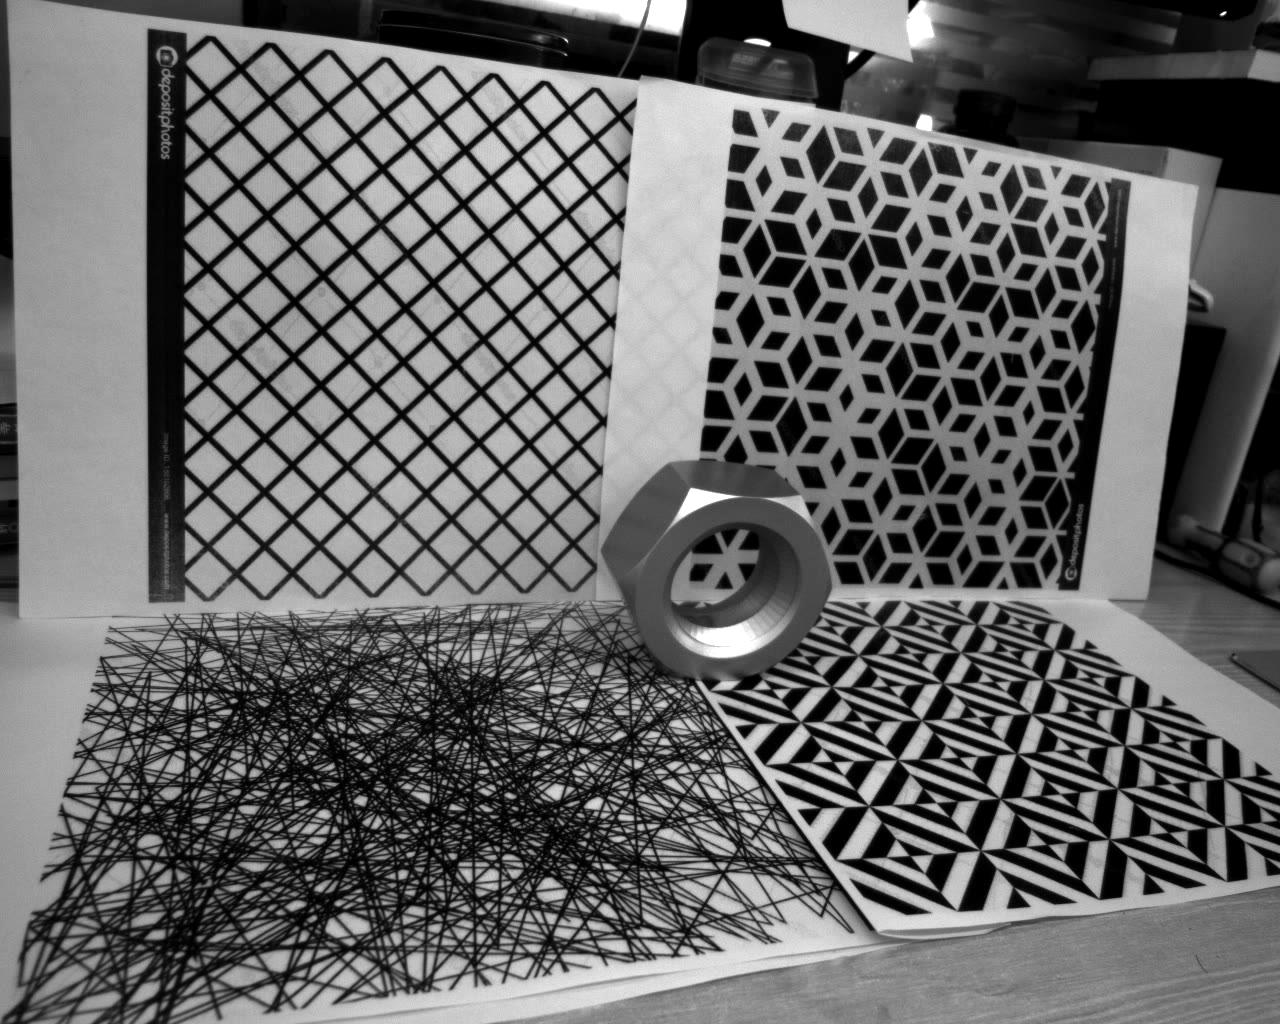
\includegraphics[height=3.8cm]{nut_yuan_3}
    \vskip 1pt
    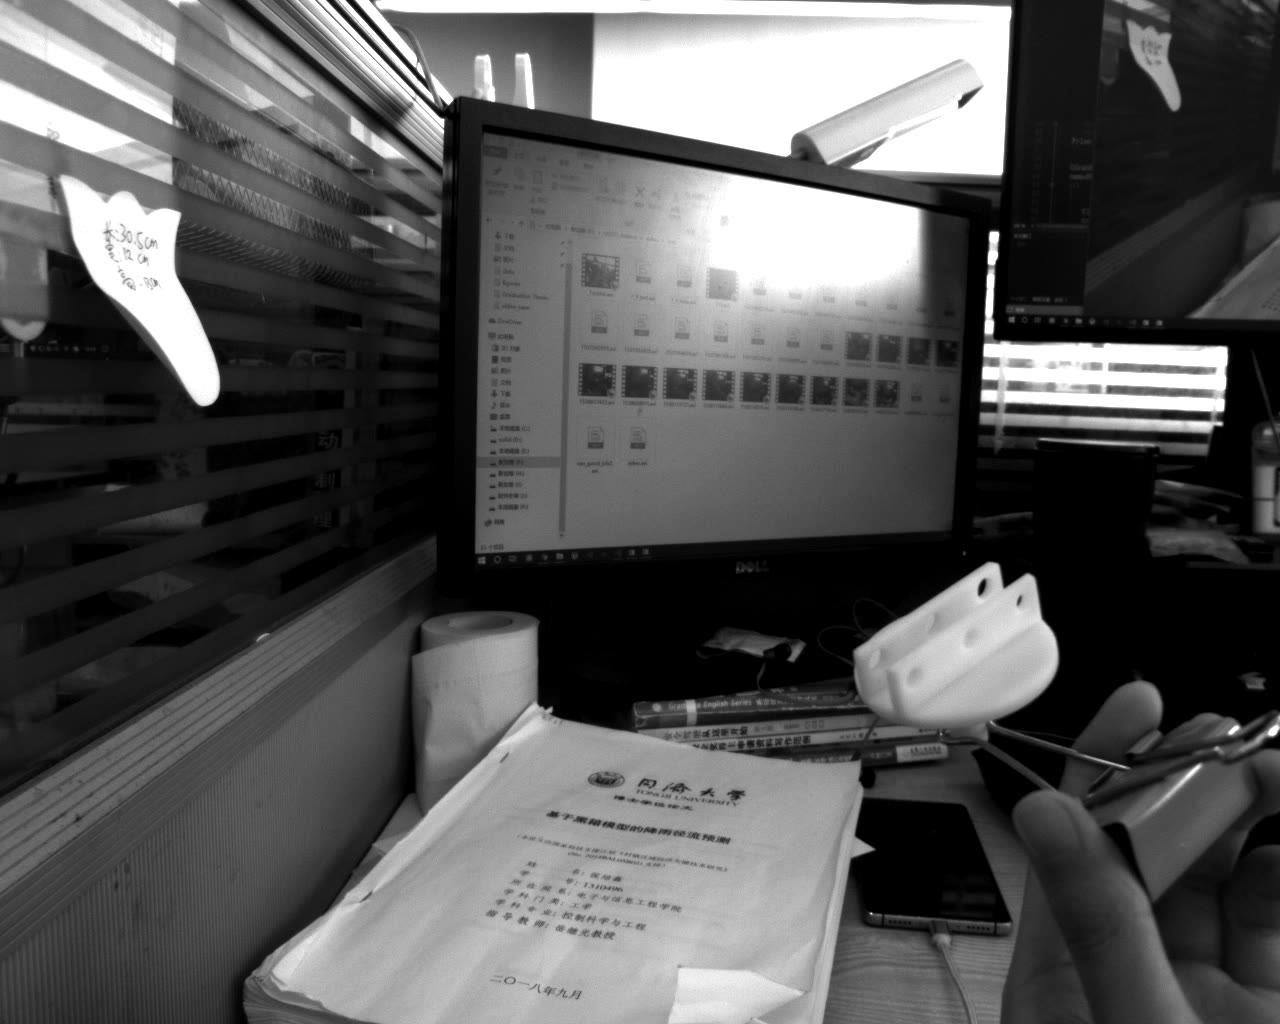
\includegraphics[height=3.8cm]{san_yuan_1}
    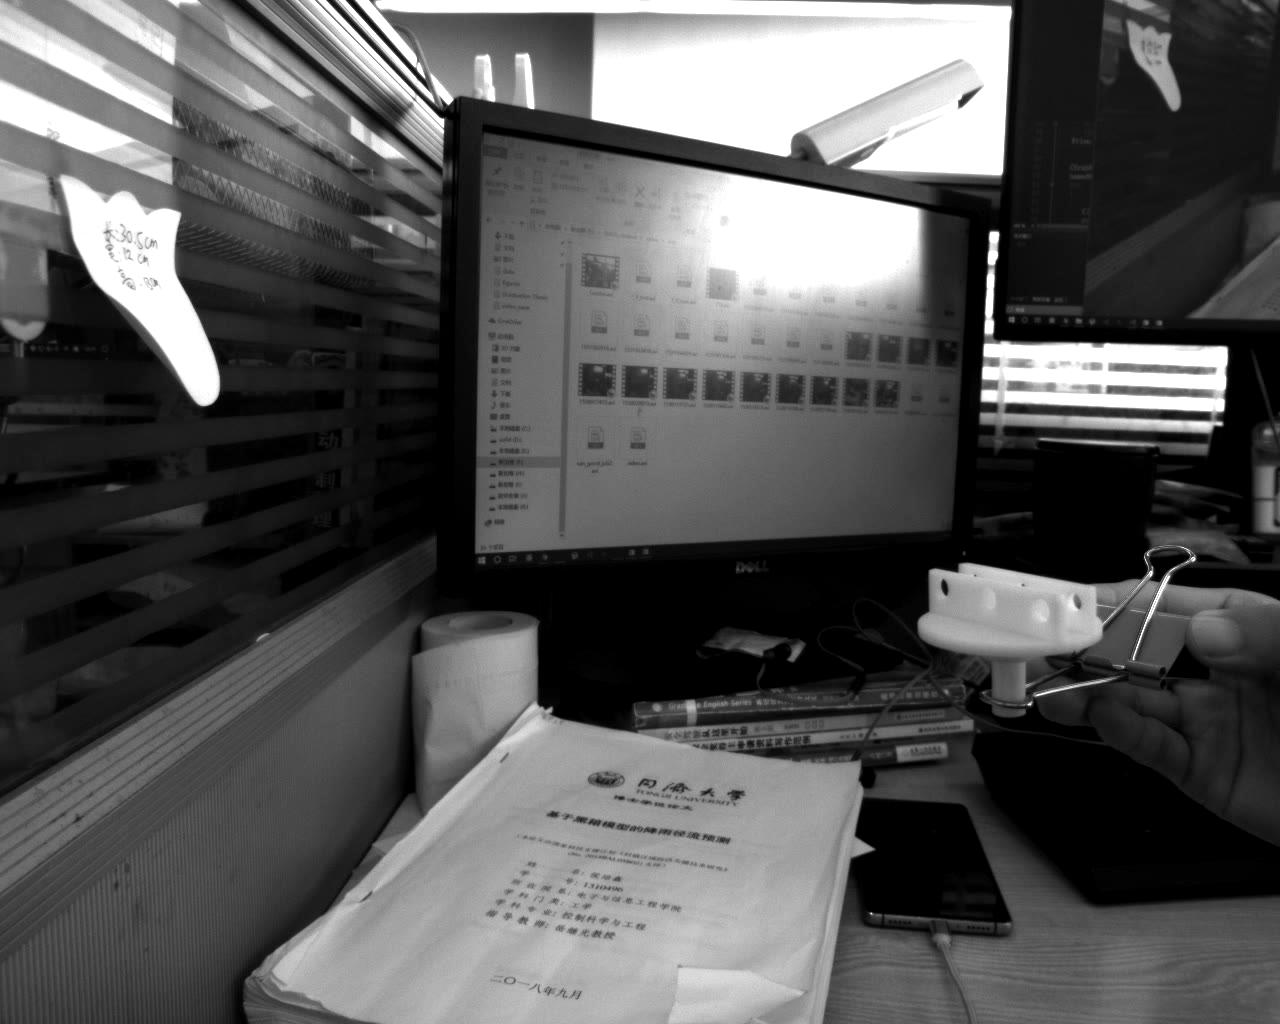
\includegraphics[height=3.8cm]{san_yuan_2}
    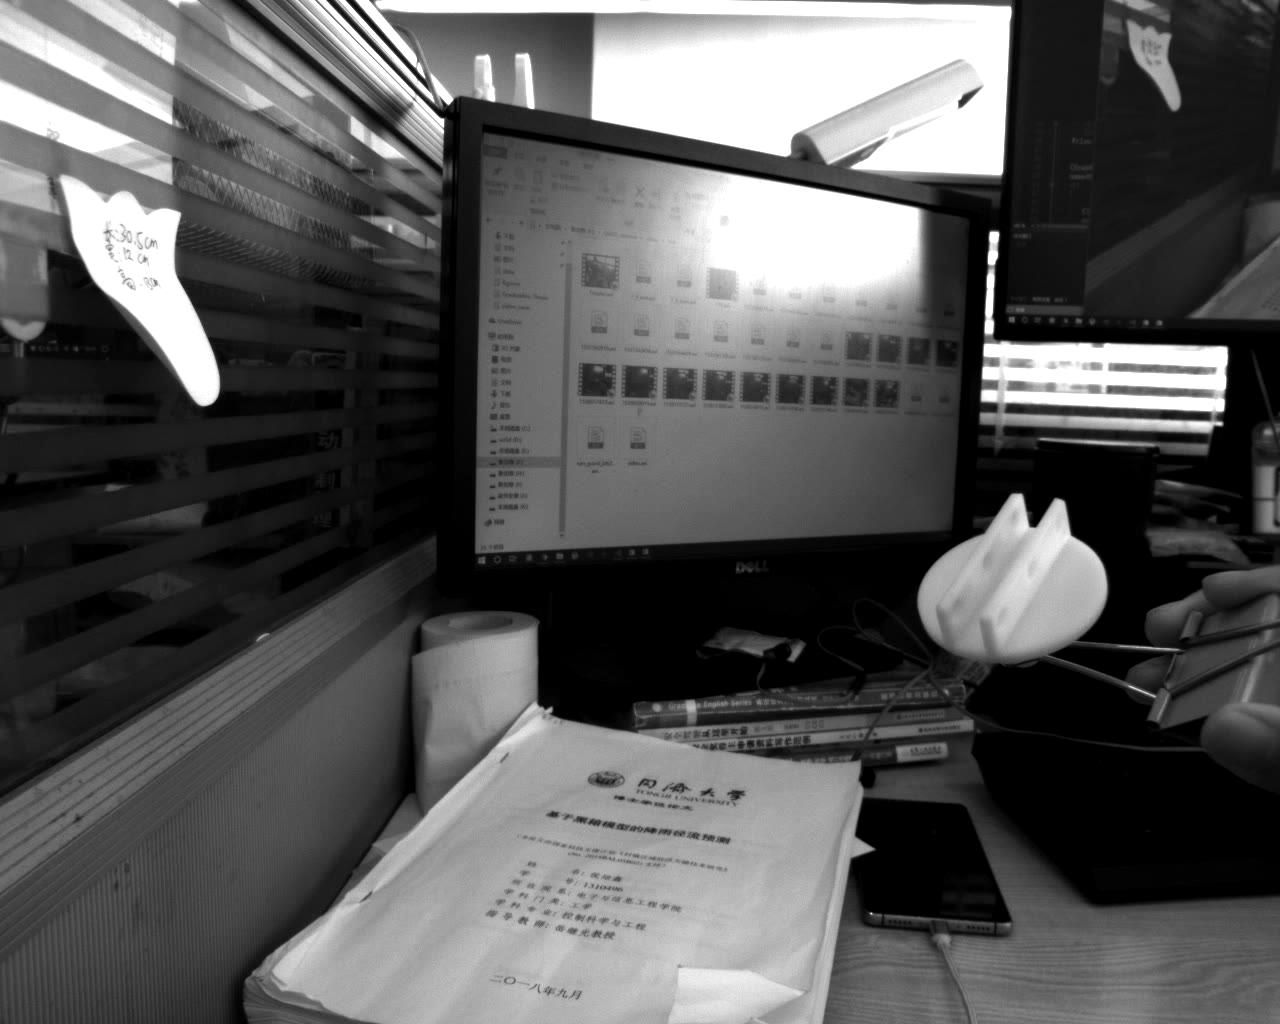
\includegraphics[height=3.8cm]{san_yuan_3}
    \vskip 1pt
    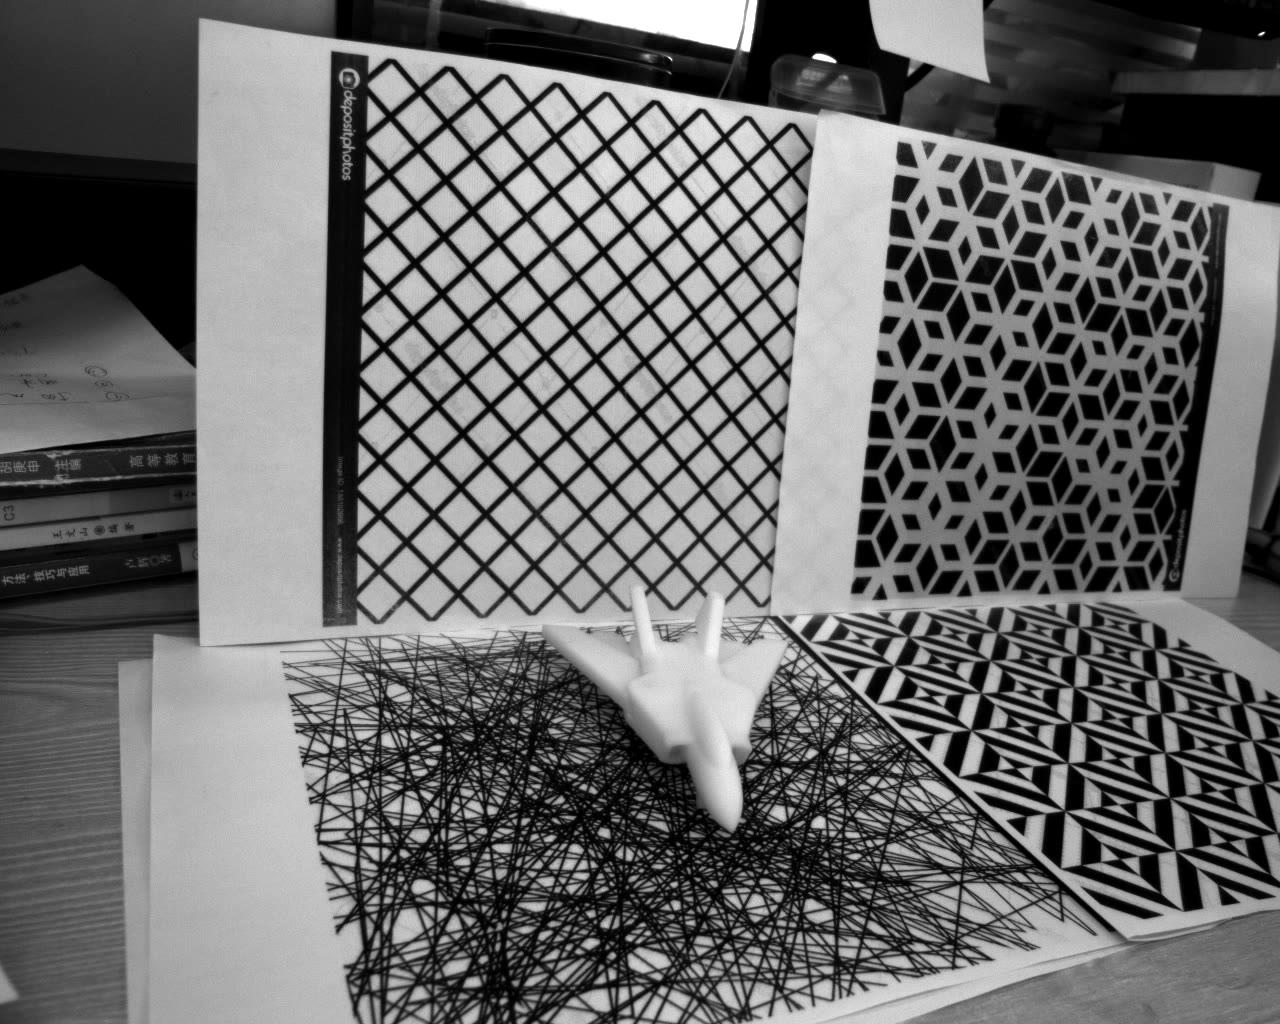
\includegraphics[height=3.8cm]{jet_yuan_3}
    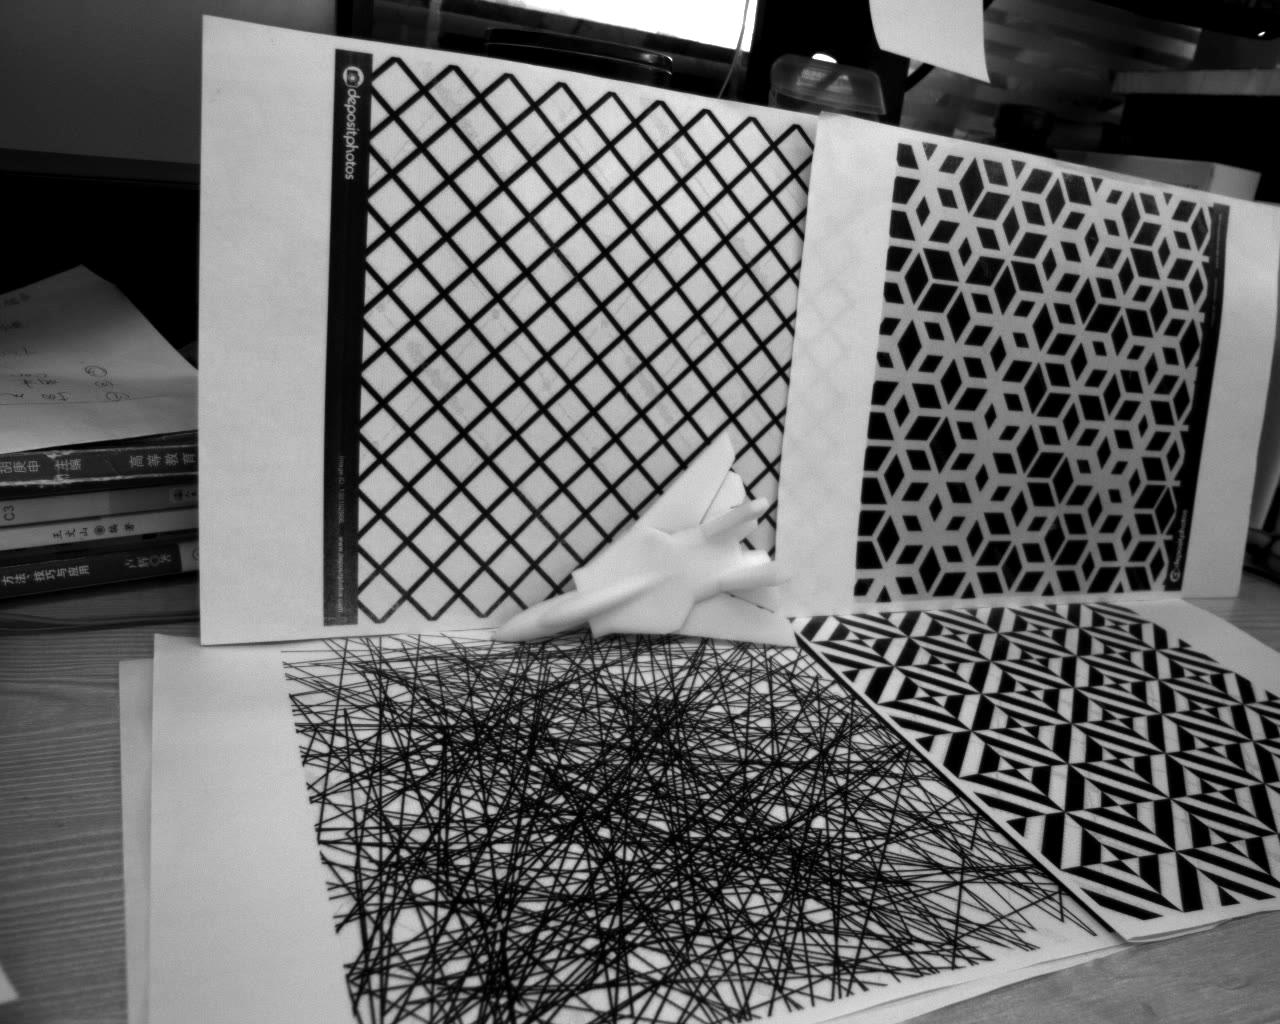
\includegraphics[height=3.8cm]{jet_yuan_2}
    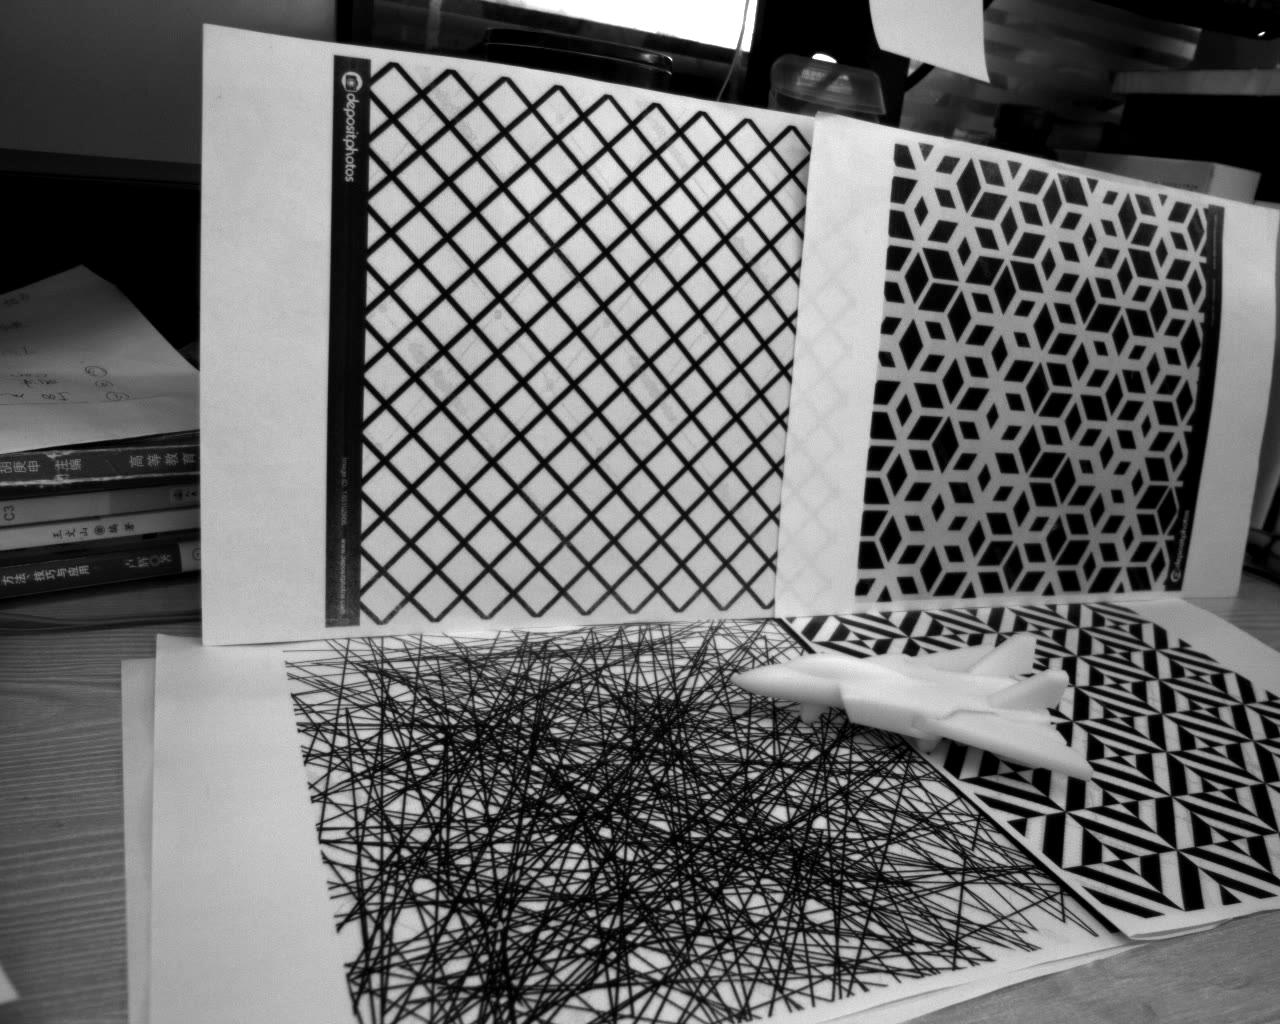
\includegraphics[height=3.8cm]{jet_yuan_1}
    \caption{场景原始灰度图像}
    \label{fig:chap03:raw_gray_imgs}
    \end{figure}

但由于贫纹理物体在灰度图像中的特征不够明显,若直接提取灰度图像作为训练数据,获得的模型难以区分目标物体与背景特征,易受复杂背景的影响。
因此本文并不保存灰度图像作为检测数据库,而使用章节~\ref{sec:Edge Point Mapping}~中研究的~DCM~张量作为图像数据进行保存,该张量中所有像素点的值代表距离该像素点最近的图像边缘点的二维欧拉距离,因此距离边缘点近的点,灰度值低,图像偏暗,而距离
边缘点远的点,灰度值高,图像偏亮,如图~\ref{fig:chap03:DCM_tensor_object_imgs}~为利用分割后的灰度图像进行~DCM~张量提取的结果图。由图可知,通过~DCM~张量变换后的图像能够更加明显地表明目标物体的边缘关系。
因此本文使用所选图像区域对场景图片的~DCM~张量进行分割,提取仅包含物体边缘的图像区域作为检测数据库的正样本。

为降低检测模型的误检率,需要准备一定数量的负样本。本文使用追踪算法获得每帧图像中目标物体的图像范围后,使用随机的方法在当前图像的其他区域,截取相同大小的~DCM~张量图像作为负样本保存。
具体的生成方法为,在图像范围内随机寻找点~$P'(x',~y')$,以该点作为图像截取矩阵的左顶点,使用正样本相同的尺寸截取图像,保存作为负样本。
为保证负样本图像不过多的包含目标物体边缘特征,需规定点~$P'$~不在如图~\ref{fig:chap03:neg_dataset_range}~所示的红色矩形范围内。该图中的绿色矩形即为选定的正样本截取范围,其左顶点即为点~$P$,
红色矩形是以~$P$~点为中心,长宽分别为~$(\frac{1}{3}leng\_x,~\frac{1}{3}leng\_y)$~的图像区域。所截取的负样本示例如图~\ref{fig:chap03:neg_img}~所示。负样本中包含了大量背景的边缘信息,训练的
检测模型将分析背景特征与目标物体特征的异同,以将两者区别。负样本中存在部分图片包含目标物体的一部分特征,通过这类图片,能够使模型有效区分包含物体所有特征以及部分特征的图片,并将包含所有特征的图片返回结果真,
仅包含部分特征的图片返回结果假,有效降低误检率。

\begin{figure}[t] %[h]
  \centering%
  %%\subcaptionbox{目标物体图像区域\label{fig:chap03:area_interesting}}[\linewidth]{%    
    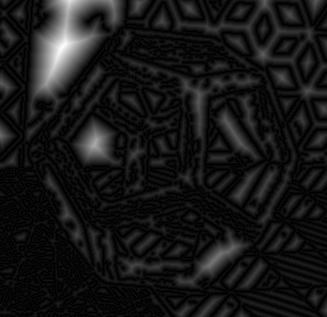
\includegraphics[height=2cm]{DCM_ball_1}\hspace{0.5em}
    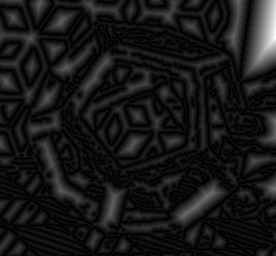
\includegraphics[height=2cm]{DCM_ball_2}\hspace{0.5em}
    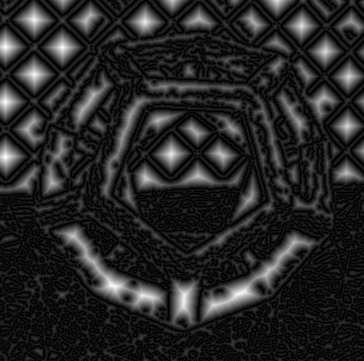
\includegraphics[height=2cm]{DCM_ball_3}\hspace{0.5em}
    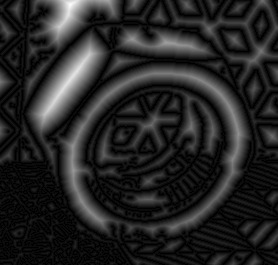
\includegraphics[height=2cm]{DCM_nut_1}\hspace{0.5em}
    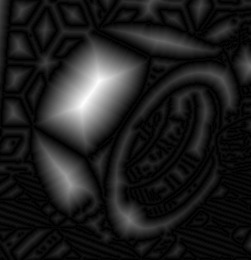
\includegraphics[height=2cm]{DCM_nut_2}\hspace{0.5em}
    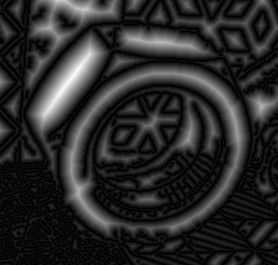
\includegraphics[height=2cm]{DCM_nut_3}
    \vskip 1.5pt
    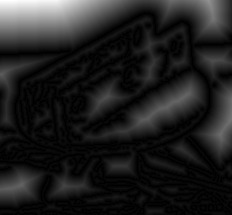
\includegraphics[height=1.8cm]{DCM_san_1}\hspace{1em}
    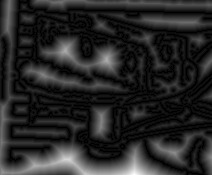
\includegraphics[height=1.8cm]{DCM_san_2}\hspace{1em}
    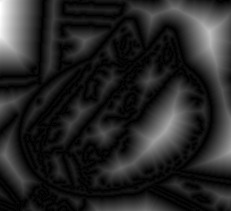
\includegraphics[height=1.8cm]{DCM_san_3}\hspace{1em}
    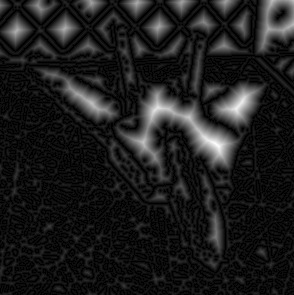
\includegraphics[height=1.8cm]{DCM_jet_3}\hspace{1em}
    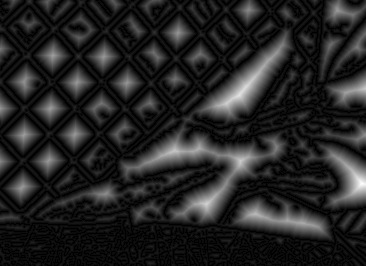
\includegraphics[height=1.8cm]{DCM_jet_2}\hspace{1em}
    \vskip 1.5pt
    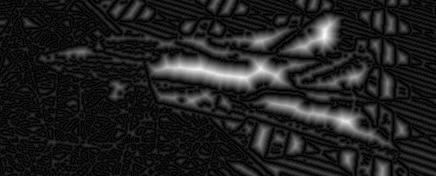
\includegraphics[height=1.8cm]{DCM_jet_1}
  \caption{目标物体~DCM~张量图}
  \label{fig:chap03:DCM_tensor_object_imgs}
  \end{figure}
\begin{figure}[t] %[h]
  \centering%
    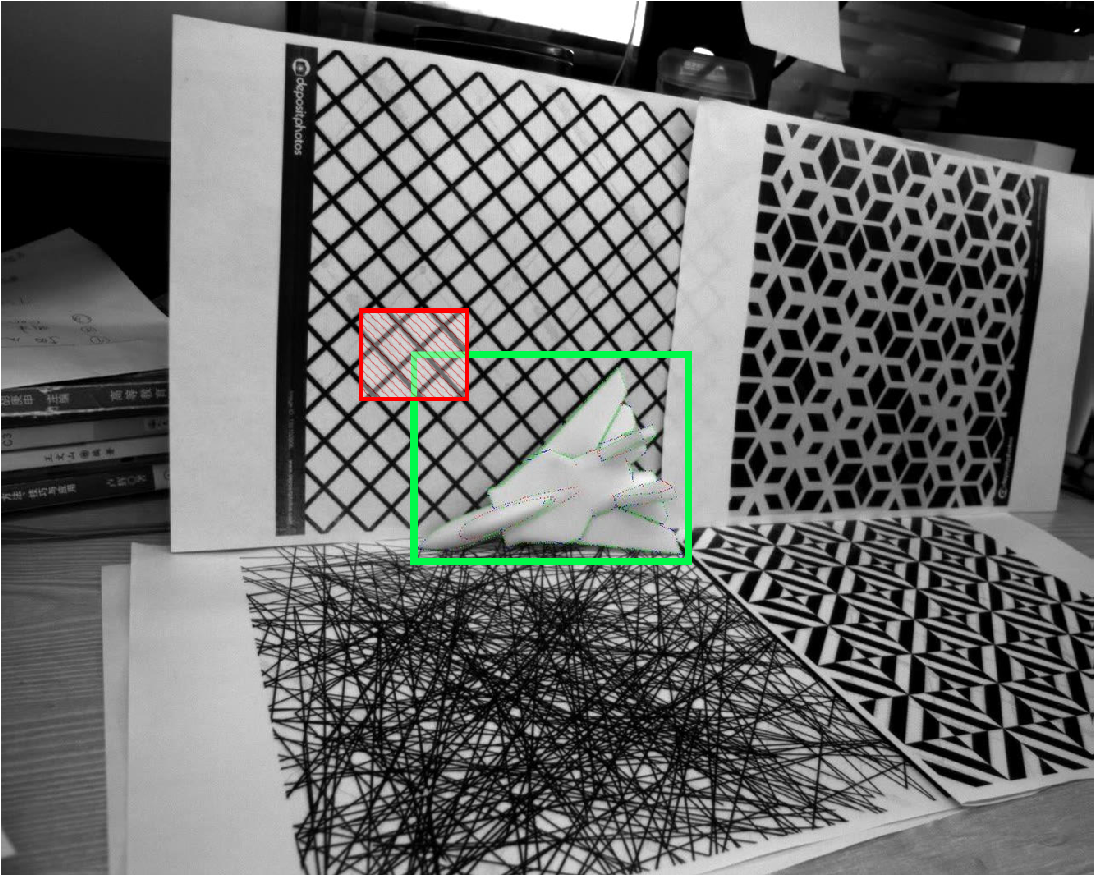
\includegraphics[height=9cm]{neg_dataset_p_point}
  \caption{负样本顶点图像区域选择示意图}
  \label{fig:chap03:neg_dataset_range}
  \end{figure}
  \begin{figure}[t] %[h]
    \centering%
    %%\subcaptionbox{目标物体图像区域\label{fig:chap03:area_interesting}}[\linewidth]{%    
      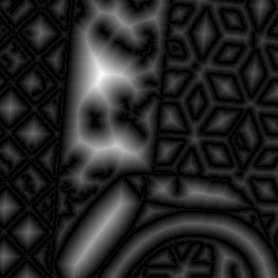
\includegraphics[height=2.7cm]{neg1}\hspace{0.2em}
      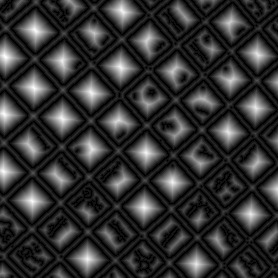
\includegraphics[height=2.7cm]{neg2}\hspace{0.2em}
      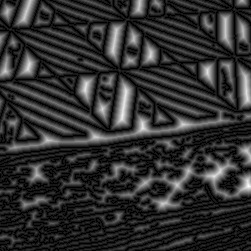
\includegraphics[height=2.7cm]{neg3}\hspace{0.2em}
      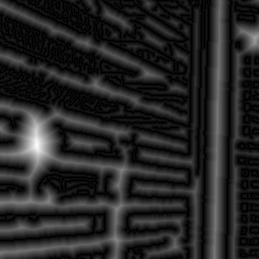
\includegraphics[height=2.7cm]{neg4}\hspace{0.2em}
      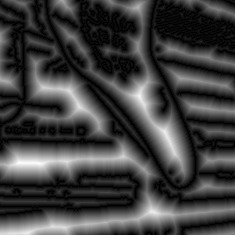
\includegraphics[height=2.7cm]{neg5}
      \vskip 1.5pt
      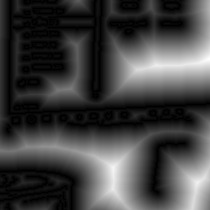
\includegraphics[height=2.7cm]{neg6}\hspace{0.2em}
      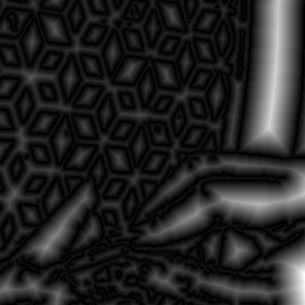
\includegraphics[height=2.7cm]{neg7}\hspace{0.2em}
      \includegraphics[height=2.7cm]{neg8}\hspace{0.2em}
      \includegraphics[height=2.7cm]{neg9}\hspace{0.2em}
      \includegraphics[height=2.7cm]{neg10}
    \caption{负样本示例图}
    \label{fig:chap03:neg_img}
    \end{figure}

由于物体在不同姿态下的边缘特征相差较大,使用单一模型对物体进行所有姿态下的检测难度较大,因此本文将同一物体在不同姿态下的特征作分类,将不同姿态下的特征作为单独的检测类以训练模型。
该方法能够降低检测模型的训练难度,提高
正检率,并且在检测阶段即将物体姿态进行粗分类,能够降低后续姿态回归的难度,提高追踪结果的精度。为实现物体不同姿态的粗分类检测,需要准备物体在不同分类类别下的训练样本。首先根据目标物体模型的对称特点,选定
其粗分类姿态的数量,并通过姿态分析得到不同分类下的姿态分隔规则,通过该规则对所有正样本进行分类,由此得到姿态粗分类下的正样本数据库,具体信息如表~\ref{table:chap03:detect_dataset}~所示,其中
~$r_x,~r_y,~r_z$~分别代表物体绕相机坐标系~$x,~y,~z$~轴旋转的欧拉角幅度值。所有物体的粗分类数量相加等于~10,因此在完成所有数据库图片位姿粗分类后,赋予所有类别一个独立的~$1\sim 10$~的数字,
作为该检测分类的真值,将负样本的真值设置为~$0$,由此完成检测数据库的构建。

\begin{table}%[h]
  \centering
  \caption{检测数据库统计}
  \label{table:chap03:detect_dataset}
  \begin{tabular}{lccl}
    \toprule
    目标物体 & 姿态类别数 & 分隔规则 & 图片数量   \\
    \midrule
    \multirow{3}*{圆盘固定件}    & \multirow{3}*{三分类} & $-3.14\leq r_y < -1.28$ & 784\\ 
    ~    & ~ & $-1.28\leq r_y < 0.91$ & 1326 \\ 
    ~    & ~ & $0.91\leq r_y \leq 3.14$ & 733 \\ 
    \multirow{2}*{螺母}    & \multirow{2}*{两分类} & \color{blue}$1.35\leq r_x,r_y,r_z \leq 1.82~or -1.82\leq r_x,r_y,r_z \leq 1.35$ & \color{blue}1126\\ 
    ~    & ~ & \color{blue}其余 & \color{blue}785 \\ 
    \multirow{3}*{飞机模型}    & \multirow{3}*{三分类} & $0.54 < r_x \leq 3.14$ & 1285\\ 
    ~    & ~ & $-0.54 < r_x \leq 0.54$ & 891 \\ 
    ~    & ~ & $-3.14\leq r_x < -0.54$ & 656 \\ 
    \multirow{2}*{五边形球体}    & \multirow{2}*{两分类} & \color{blue}$\frac{n }{5}\pi + 0.63 \leq r_x,r_y,r_z \leq \frac{n}{5}\pi - 0.63$ & \color{blue}981\\ 
    ~    & ~ & \color{blue}其余 & \color{blue}875 \\ 
    负样本   & - & - & 9442\\ 
    \bottomrule
  \end{tabular}
\end{table}

\subsection{位姿回归数据库}
\label{sec:dataset_tracking}
检测算法能够获得目标物体在图像平面的位置,但仍然无法确定物体相对于相机的位姿关系。因此本文还需使用其他方法获得物体相对于相机的精确位姿。
由于物体相对于相机坐标系的平移向量直接关系到其在相机视野中的位置,通过相机投影模型可知,当目标平移向量发生改变时,其在图像平面的位置也会发生变化。因此本文拟使用目标物体在图像平面的位置作为特征,训练回归模型,
得到其相对于相机坐标系的平移向量。本节将研究用以训练该模型的数据库构建方法。

\begin{figure}[t] %[h]
  \centering%
  %%\subcaptionbox{目标物体图像区域\label{fig:chap03:area_interesting}}[\linewidth]{%    
    \includegraphics[height=3.8cm]{regre1}
    \includegraphics[height=3.8cm]{regre2}
    \includegraphics[height=3.8cm]{regre3}
    \vskip 1.5pt
    \includegraphics[height=3.8cm]{regre4}
    \includegraphics[height=3.8cm]{regre5}
    \includegraphics[height=3.8cm]{regre6}
  \caption{回归数据库示意图}
  \label{fig:chap03:regre_dataset}
  \end{figure}
\begin{table}[t]
  \centering
  \caption{回归数据库统计}
  \label{table:chap03:regre_dataset}
  \begin{tabular}{lcc}
    \toprule
    目标物体 & 姿态类别数 & 图片数量   \\
    \midrule
    \multirow{3}*{圆盘固定件}    & \multirow{3}*{三分类} & 329\\ 
    ~    & ~ & 447 \\ 
    ~    & ~ & 368 \\ 
    \multirow{2}*{螺母}    & \multirow{2}*{两分类} & \color{blue}486\\ 
    ~    & ~ & \color{blue}567 \\ 
    \multirow{3}*{飞机模型}    & \multirow{3}*{三分类} & 428\\ 
    ~    & ~ & 378 \\ 
    ~    & ~ & 455 \\ 
    \multirow{2}*{五边形球体}    & \multirow{2}*{两分类} & \color{blue}394\\ 
    ~    & ~  & \color{blue}356 \\ 
    \bottomrule
  \end{tabular}
\end{table}

首先,目标物体在图像中的位置,即通过上节中介绍的光栅点投影方法得到,如图~\ref{fig:chap03:neg_dataset_range}~中的绿色框即表示物体在图像中的位置,通过保存该框的左顶点坐标
~$P(x,~y)$~以及该框的长宽~$(leng\_x,~leng\_y)$~以作为图像位置特征。其次,物体在不同位姿下的图像特征差距较大,例如图~$\ref{fig:chap03:area_interesting}$~中的飞机模型,其三种位姿下的
检测框尺寸差距明显,因此使用同一模型对不同粗分类位姿下的平移向量回归将造成很大误差,所以将目标物体的粗分类类别作为输入特征一同训练模型,使模型能够根据粗分类的类别得到不同的回归结果。最后,通过追踪算法得到的
物体平移向量~$[t\_x,~t\_y,~t\_z]$~作为真值,由此完成回归数据库构建。

为使得回归模型能够准确得到目标物体在各种图像位置下的平移向量,需使回归数据库中尽量多的包含各种位置下对应的向量真值。如图~\ref{fig:chap03:regre_dataset}~所示,在录制视频时,应使目标物体活动范围扩大,尽量多的遍历
相机采集图像的各个区域,提高回归数据库的完整性。回归数据库的统计信息如表~\ref{table:chap03:regre_dataset}~所示。

\section{CG~渲染真值数据库生成}
\label{sec:dataset_engine}
在真实环境中,要获得目标相对于相机的精确位姿十分困难,通过姿态传感器等的测量方法存在较大误差,并且实现成本高昂。而现有数据库存在数量少、精度低的缺点,因此本文将研究利用计算机图像学~(Computer Graph,简称:~CG~)~的方法渲染图片以替代传统
数据集的方法。使用~CG~方式生成数据库的优势有:
\begin{enumerate}[(1)] 
  \item 不需要配置实体设备,如相机、光源、实物模型以及真值测量传感器等,大大降低了数据采集的成本和难度;
  \item 可以任意配置光照、背景,模型现实场景中的各种明暗环境,能够轻松切换背景图像,获得不同环境干扰下的视频数据;
  \item 可以灵活调整物体与相机的相对位姿,使得数据库包含丰富的位姿状态,获得物体各种位姿状态下的视频数据;
  \item 通过渲染引擎对场景的解析,能够获得物体相对相机的精确位姿真值,对比人工测量精度更高,也更方便。
\end{enumerate}

本文将研究使用~3ds Max~的~V-Ray~渲染引擎构建目标物体位姿数据库的方法,本节将对比两种渲染引擎的结果,讨论各自的优缺点,并在最后得到虚拟的位姿数据库。
该数据库将包含渲染得到的虚拟视频,以及每一帧图像中所有物体相对于相机的位姿真值。该结果将作为真值数据以用于追踪算法的精度测量。
\subsection{渲染场景搭建}
\label{sec:dataset_blender}
本文使用~3ds Max~软件平台搭建渲染环境。3ds Max~是一个专业的~3D~计算机图形程序,用于制作~3D~动画、模型以及图像,具有强大的建模功能和灵活的插件构架,用户能够使用脚本定制模型、光照以及各部件的运动轨迹,方便得到
预定的效果。它常被用于动画生成、商业建筑可视化等领域,在动态模拟、粒子系统、光能传递以及模型的创建和渲染方面有着强大的功能。
\begin{figure}[t] %[h]
  \centering%
  \includegraphics[height=7cm]{cg_plane}
\caption{渲染场景搭建}
\label{fig:chap03:cg_rander_build}
\end{figure}
\begin{figure}[t] %[h]
  \centering%
  %%\subcaptionbox{目标物体图像区域\label{fig:chap03:area_interesting}}[\linewidth]{% 
  \subcaptionbox{渲染背景原始图片\label{fig:chap03:cg_raw_bkg}}{   
    \includegraphics[height=4cm]{raw_bkg_2}\hspace{0.4em}
    \includegraphics[height=4cm]{raw_bkg_1}\hspace{0.4em}
    \includegraphics[height=4cm]{raw_bkg_3}}
    \vskip0.3cm
    \subcaptionbox{渲染背景~DCM~张量图\label{fig:chap03:cg_dcm_bkg}}{
    \includegraphics[height=4cm]{DCM_bkg_2}\hspace{0.4em}
    \includegraphics[height=4cm]{DCM_bkg_1}\hspace{0.4em}
    \includegraphics[height=4cm]{DCM_bkg_3}}
  \caption{渲染视频背景图}
  \label{fig:chap03:cg_bcg_img}
  \end{figure}

本文所搭建的场景如图~\ref{fig:chap03:cg_rander_build}~所示,将多个目标物体放置于平台之上,保持所有物体都能出现在相机视野中,这样渲染一次视频即能获得针对所有物体的视频数据库。
通过切换平台的贴纸即能方便地改变模型所处环境的背景图像,如图~\ref{fig:chap03:cg_bcg_img}~所示为本文所选的不同背景图片及其~DCM~张量提取图,通过使用金属板、传送带纹理以及木纹作为渲染视频时的背景图片,以模拟
真实场景中出现的背景干扰。
相机选择目标相机,该相机包含一个视点坐标,在相机位置发生变化时,视角将始终以该视点作为图像的中点,通过将视点放置于平面中心,保证所有物体始终处在相机视野内。
之后构造圆线框作为相机的运动轨迹,随着视频帧数的前进,相机将会匀速在该圆环上运动,运动过程中相机的位置和姿态都在变化,也即使得物体相对于相机的位姿也会因此改变。渲染整个运动过程中相机视野内的图像,并计算每帧图像对应的相对位姿关系,
以作为虚拟数据库的真值。
目标相机的视点位置、轨迹圆环的半径、轨迹圆环距离平台的高度以及目标物体的位姿都会影响整个视频中,物体与相机的相对位姿关系。由此通过~CG~渲染的方法能够得到大量不同位姿下的视频数据。

\begin{figure}[b] %[h]
  \centering%
  %%\subcaptionbox{目标物体图像区域\label{fig:chap03:area_interesting}}[\linewidth]{% 
  \subcaptionbox{局部坐标系方向示意图\label{fig:chap03:obj_axis}}{   
    \includegraphics[height=4cm]{camera_obj}\hspace{0.4em}
    \includegraphics[height=4cm]{jet_gongzuo}}
    \vskip0.3cm
    \subcaptionbox{世界坐标系方向示意图\label{fig:chap03:world_axis}}{
    \includegraphics[height=4cm]{camera_shijie}\hspace{0.4em}
    \includegraphics[height=4cm]{jet_shijie}}
  \caption{坐标系方向差异示意图}
  \label{fig:chap03:diff_axis}
  \end{figure}


\subsection{位姿真值获取}
\label{sec:dataset_3ds_max}
在~3ds Max~平台中,所有物体以及相机都属于场景中的部件,每一个部件都拥有各自的局部坐标系,此外场景还拥有唯一的世界坐标系,局部坐标系与世界坐标系的原点以及方向都不相同,其方向差异如图~\ref{fig:chap03:diff_axis}~所示。
物体在~3ds Max~中的位置和姿态表示其局部坐标系相对于世界坐标系的平移向量以及旋转向量,假设飞机模型的局部坐标系为~$C_j$,相机的局部坐标系为~$C_m$,世界坐标系为~$C_g$,假设~$R$~代表坐标系间的旋转矩阵,$R_{ab}$~代表坐标系~$C_a$~相对于
坐标系~$C_b$~的旋转矩阵,假设~$\textrm{T}$~代表坐标系间的平移向量,$\textrm{T}_{ab}$~代表坐标系~$C_a$~相对于坐标系~$C_b$~的平移向量。在~3ds Max~中旋转关系使用角度制的欧拉角表示,而平移向量的单位为毫米。

首先,物体的姿态信息在~3ds Max~中是利用欧拉角表示的,其旋转轴顺序为~ZXY,通过式~(\ref{equ:chap03:eul2rot})~将欧拉角变换为旋转矩阵。
\begin{equation}
  \label{equ:chap03:eul2rot}
  R(\alpha, \beta, \gamma)=\left[   
  \begin{matrix}
    c_1c_3+s_1s_2s_3 & c_3s_1s_2-c_1s_3 & c_2s_1\\
    c_2s_3 & c_2c_3 & -s_2 \\
    c_1s_2s_3-s_1c_3 & s_1s_3+c_1c_3s_2 & c_1c_2
  \end{matrix}
  \right]
\end{equation}
其中,$c_1=\cos(\alpha),s_1=\sin(\alpha), c_2=\cos(\beta),s_2=\sin(\beta), c_3=\cos(\gamma),s_3=\sin(\gamma)$。
之后先将物体坐标系变换到世界坐标系,旋转矩阵为~$R_{jg}$,再将世界坐标系变换到相机坐标系,旋转矩阵为~$R_{gm}$,再根据旋转矩阵求逆的方法可得物体相对于相机的旋转矩阵如式~(\ref{equ:chap03:rot_obj_cam})~所示:
\begin{equation}
  \label{equ:chap03:rot_obj_cam}
  R_{jm} = R_{jg}*R_{gm} = -R_{gj}*R_{gm} = R_{gj}^{T}*R_{gm}
\end{equation}
其中~$R_{gj}$~以及~$R_{gm}$~能够由~3ds Max~平台读取的欧拉角变换得到。由此得到~$R_{jm}$~代表~3ds Max~平台上目标物体相对于相机坐标系的旋转矩阵,但追踪算法使用的相机坐标系与渲染引擎的相机坐标系在~$X$~轴上
相差~$180^\circ$,因此最终的旋转矩阵真值数据如式~(\ref{equ:chap03:tracking_rot_angle})~所示。
\begin{equation}
  \label{equ:chap03:tracking_rot_angle}
  R'_{jm} = R_{jm}*R_{\pi x}
\end{equation}
其中~$R_{\pi x}$~代表在~X~轴上的旋转以对齐两个平台的相机坐标系。平移向量的真值~$\textrm{T}_{jm}$~能够直接由~3ds Max~平台脚本~distance \$[j] \$[m]~获得,在此不再叙述。

\subsection{位姿真值数据库生成}
\label{sec:dataset_compare}
完成场景搭建以及位姿真值计算后,本文使用~V-Ray~渲染引擎对相机视野内的图像进行渲染。该引擎是一种使用全局照明算法的渲染引擎,通过从摄像头发射辐射状的搜索射线,以确定图像平面中每一个像素点
与场景中的三维空间点的对应关系,之后针对所有可是范围内的三维点,计算能够到达该点的光源强度,并根据该点的材质,确定其最终的现实效果。其主要渲染参数有细分值以及光照计算方法,细分值决定了渲染结果的细腻程度,
该值过低会导致图像锯齿感明显,提高该值能够使得图像过渡更加光滑,但会增加渲染耗时,本文选择细分值为~10。光照的计算方法主要有两种,一种是直接法,另一种为间接法。直接法又分为一次反射、二次反射以及多次
反射,通过追踪光线并计算其反射来确定所有视野范围内的亮度,考虑的反射次数越多,场景越亮,直接法计算耗时较多,比较适合于光照复杂的环境;间接法并不计算所有像素点的亮度,而是选择一段亮度连续变化的区域,
通过计算该区域两个端点的亮度以均匀填补中间点的亮度。间接法计算快速,并且针对照明环境较为简单的场景,其亮度变化更加均匀,因此本文选用间接法对场景亮度进行计算。 
\begin{figure}[t] %[h]
  \centering%
    \includegraphics[height=3.6cm]{wood_cg_1}
    \includegraphics[height=3.6cm]{raw_cg_1}
    \includegraphics[height=3.6cm]{raw_cg_3}
    \vskip 1.5pt
    \includegraphics[height=3.6cm]{wood_cg_2}
    \includegraphics[height=3.6cm]{raw_cg_2}
    \includegraphics[height=3.6cm]{raw_cg_4}
  \caption{渲染背景切换}
  \label{fig:chap03:change_bkg_img}
  \end{figure}

  \begin{comment}
  \begin{figure}[t] %[h]
    \centering%
      \includegraphics[height=2.65cm]{tiplier70}
      \includegraphics[height=2.65cm]{tiplier130}
      \includegraphics[height=2.65cm]{tiplier210}
      \includegraphics[height=2.65cm]{tiplier300}
    \caption{光照改变示意图}
    \label{fig:chap03:change_ray}
    \end{figure}
    之后本文还调整了场景的光源强度以渲染不同光照下的视频数据,如图~\ref{fig:chap03:change_ray}~所示,
该数据将被用于测试光照强度对追踪算法的影响。
  \end{comment}

切换不同桌面背景的渲染结果如图~\ref{fig:chap03:change_bkg_img}~所示,选择不同的纹理以模拟系统所处的不同环境,由于所要测试的追踪算法是利用~DCM~张量以实现匹配寻优,
而~DCM~张量是通过场景边缘图像提取得到。因此本文选择含有较多边缘纹理的背景,该类背景对追踪算法的干扰较强,对系统的稳定性将提出更高的要求。

\section{本章小结}
\label{sec:summary}
本章研究了检测数据库的构建方法,在灰度图像中利用追踪算法定位目标物体,并裁剪~DCM~张量图得到仅包含目标物体的部分。之后根据目标物体的模型对称性质,将检测数据库按照其位姿作粗分类,不同粗分类的物体含有不同的
标签,保存图像及其标签以备后续算法的训练。为训练位姿估计模型,本章继续研究了位姿回归数据库的构建方法,通过追踪算法获得每一帧图像中物体相对于相机的位姿,之后利用相机投影模型得到模型光栅点的图像位置,根据光栅点的图像坐标确定物体检测框,保存该检测框的顶点坐标、长宽尺寸
以及对应时刻的相对位姿关系,以备后续位姿回归模型的训练。

之后研究基于计算机图像学的虚拟视频渲染方法,利用该技术制作位姿真值数据库。主要讨论了场景的搭建和背景的选择方法,并研究了调整相机视点、运动的轨迹以及目标物体的姿态以得到不同的相对位姿。
使用该方法能够灵活地调整物体在相机视野中的位置和姿态,大大降低了数据库的制作成本。之后继续研究在~3ds Max~平台上获得物体相对于相机精确位姿关系的方法,使用该方法能够快速准确地得到每一帧图像中物体的相对位姿,相比真实环境中的测量方法
精度更高。最后对比了不同光照、不同背景图像的数据库视频,将所有渲染得到的视频及其位姿真值保存,以对追踪算法进行精度测试。